\chapter{Implementation}
\label{chapter:implementation}

This chapter addresses the main decisions taken in order to implement the hardware and software architectures presented in Chapter 3.


\section{Hardware Architecture}\label{hardware_arch_imp}


The next sections provide the implementation choices for the hardware architecture. As shown in Figure~\ref{imp:architecture_system} we require tablet to run the HUB app, HVAC control, lighting control and a \ac{BLE} beacon for user location tracking.



\begin{figure}[h]
\centering
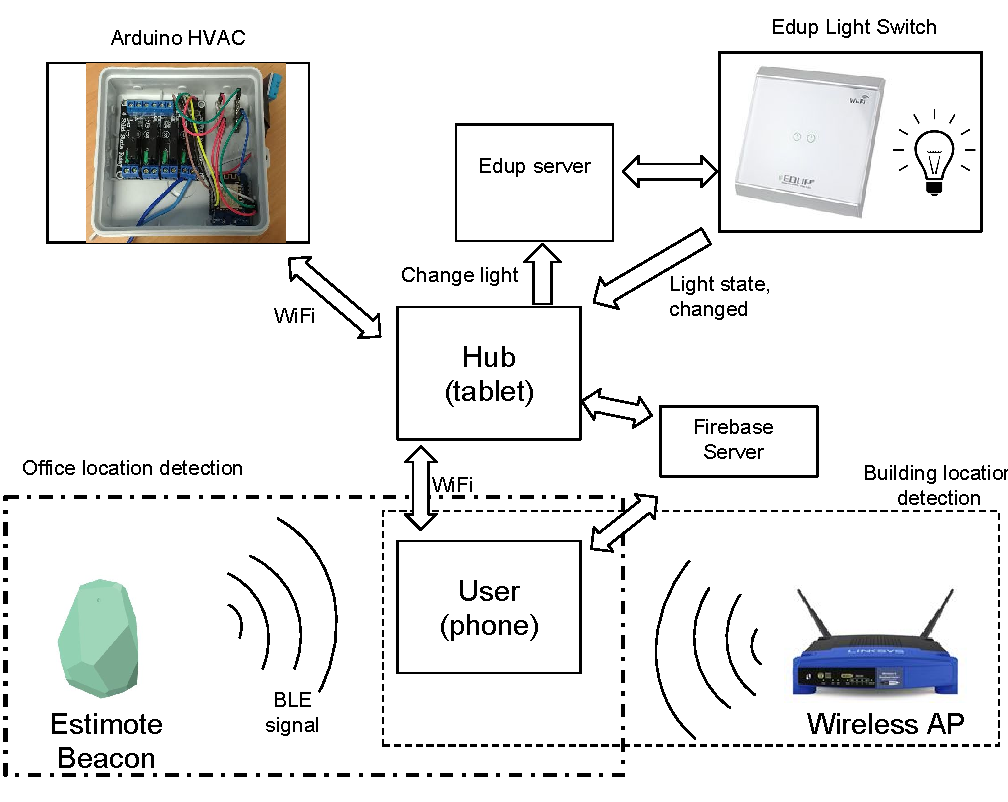
\includegraphics[width=0.8\textwidth]{Figures/harware_arch_imp}
\caption{Hardware implementation architecture}
\label{imp:architecture_system}
\end{figure}





%This chapter is divided in three main sections. In Section 4.1 the detailed hardware architecture is
%described. Each of its subsection shows the decisions taken in the selection of the components.
%Section 4.2 describes the implementation of the software architecture. This section is composed of
%several subsections that detail the software configuration and explains the developed code.
%Finally, Section 3.5 details the deployment of the system in a set of offices at IST - Taguspark.

\subsection{Tablet}

A tablet capable of supporting a range of communication protocols and with some embedded sensors must be chosen as the base for the solution.

Several tablets were taken in consideration, the decisive factors were the price, \ac{CPU} speed/cores, \ac{RAM} and finally the supported communication protocols (\ac{BLE} and \ac{WiFi} are required). These factors are important since they allow the device to easier bought (price), allow multiple parallel complex computational operations like image processing, video recording, voice recognition. Since the tablet will be communication with a client device it requires \ac{WiFi} to transfer and receive data and commands, \ac{BLE} can be used to read external sensor data such as temperature.


Table~\ref{table:tablet} shows some examples of tablets running the major operating systems with similar hardware specifications.

In terms of price Apple tablets have the largest cost, since there is such a big gap in cost the iPad Mini 4 does not fit our needs. There are many types of Windows and Android tablets with very affordable prices. The Nexus was chosen because it was developed by Google in partnership with Asus, has very good reviews and is updated to the latest android version. There are Windows tablets cheaper than the HP ENVY 8 sold by Microsoft but there were a lack of reviews so a good tablet from a big manufacturer was picked.

The Android and Windows tablets have very similar hardware specifications. So the tablet chosen was the Nexus 7 (2013) since the programmer had experience developing Android apps.


\begin{table}[]
\centering
\begin{tabular}{|l|l|l|l|l|}
\hline
\textbf{name} & \begin{tabular}[c]{@{}l@{}}Apple iPad \\ mini 4\end{tabular} & Nexus 7 2013 & \begin{tabular}[c]{@{}l@{}}HP ENVY \\ 8 Note 5009\end{tabular} \\ \hline
\textbf{CPU speed} & 1.5 GHz & 1.5 GHz & 1.44 GHz \\ \hline
\textbf{CPU cores} & 2 & 4 & 4 \\ \hline
\textbf{RAM} & 2GB & 2GB & 2GB \\ \hline
\textbf{WiFi} & \begin{tabular}[c]{@{}l@{}}yes (2.4 GHz \\ and 5 GHz)\end{tabular} & \begin{tabular}[c]{@{}l@{}}yes (2.4 GHz \\ and 5 GHz)\end{tabular} & yes (2.4 GHz) \\ \hline
\textbf{BLE} & yes & yes & yes \\ \hline
\textbf{Light sensor} & yes & yes & yes \\ \hline
\textbf{Microfone} & yes & yes & yes \\ \hline
\textbf{Speaker} & yes & yes & yes \\ \hline
\textbf{Front camera} & yes & yes & yes \\ \hline
\textbf{Size} & \begin{tabular}[c]{@{}l@{}}7.9 inches (1536 \\ x 2048 pixels)\end{tabular} & \begin{tabular}[c]{@{}l@{}}7 inches (1200 \\ x 1920 pixels)\end{tabular} & \begin{tabular}[c]{@{}l@{}}8 inches (1200 \\ x 1920 pixels)\end{tabular} \\ \hline
\textbf{Operating System} & Apple IOS 10.0.1 & Android 6.0 & Windows 10 \\ \hline
\textbf{Cost (EUR)} & 449 & 131 & 178 \\ \hline
\end{tabular}
\caption{Comparison between some tablet devices}
\label{table:tablet}
\end{table}


\subsection{HVAC control}
In order for our \ac{BAS} solution to control an \ac{HVAC} system we need to either communicate with a building central controlling unit or physically controlling the system like a thermostat does. Since many buildings don't have a central control point running some kind of server where you can control it using the internet, we went with the thermostat route.

For our smart thermostat to work we require a device capable of sending electric impulses to the \ac{HVAC} wire. 

Table~\ref{thermostat-choice} shows some commercial products and a Arduino solution.

We require a device that offers a  API in order to be controlled by our tablet, because the Sensi thermostat does not offer an official API it does not fit our requirements.

The Nest thermostat is the most popular option in the market integrated in many home automation systems, but since one of our requirements is keeping the cost low it does not fit our requirements. The path chosen was developing an Arduino solution, shown in Figure~\ref{arduino_imp}, with built in \ac{WiFi}, a relay to control the electric wires and a temperature and humidity sensor.



\begin{table}[]
\centering
\begin{tabular}{|l|l|l|l|}
\hline
\textbf{Name} & \begin{tabular}[c]{@{}l@{}}Sensi Wi-Fi \\ Thermostat\end{tabular} & \begin{tabular}[c]{@{}l@{}}Nest (3rd)\\ Thermostat\end{tabular} & \begin{tabular}[c]{@{}l@{}}Wemos D1 \\ mini Arduino + \\ Temperature Humidity \\ Sensor DHT11 + \\ Solid State Relay \\ 4 Channel + box\end{tabular} \\ \hline
\textbf{temperature/humidity} & yes & yes & yes \\ \hline
\textbf{Developer API} & no & yes & yes \\ \hline
\textbf{Cost (EUR)} & 116 & 223 & 4 + 1.5 + 6 + 1 = 12.5 \\ \hline
\end{tabular}
\caption{Differences between thermostat options.}
\label{thermostat-choice}
\end{table}


\begin{figure}[h]
\centering
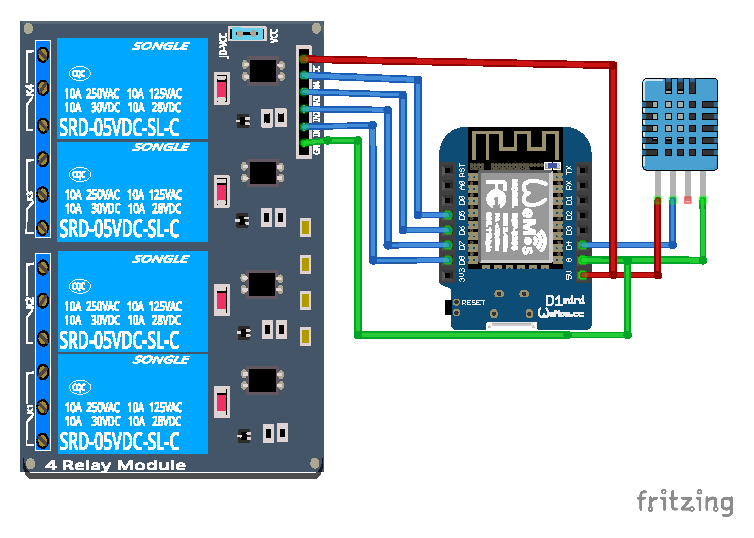
\includegraphics[width=0.7\textwidth]{Figures/arduino_imp}
\caption{Arduino HVAC circuit diagram}
\label{arduino_imp}
\end{figure}



\subsection{Lighting control}
Besides controlling the room \ac{HVAC}, we require control over the lighting system. After some research we had three options: using wireless controllable light bulbs, using some kind of Arduino/relay solution (like the thermostat) or using a wireless controllable light switch.

Table~\ref{lighting-choice} show some available options to provide lighting control.

Our lighting solution should be affordable, have a physical light switch and an API to control it. The Philips Hue is costly and does not have lights supported by our office (fluorescent tube lamp) for these reasons it does not fit our requirements.

In order for our solution to be easily deplorable it requires the least amount of assembly and soldering, an pre-built lighting product is preferable if the price range is close enough. Both the Arduino/relay and the DI-O/Arduino options have shortcomings, the first does not provide touch control and requires soldering and the latter also requires soldering in the Arduino interface side.

The lighting option chosen was the Edup Smart Light Switch, shown in Figure~\ref{edup_light_imp},  it provides a physical light switch, supports the existing infrastructure in the buildings (as long as there is a positive and negative wire in the wall socket) and is not too expensive.


Originally in Section \ref{architecture3} of the architecture, the lighting system was going to be integrated with the Arduino/\ac{HVAC} using relay actuators. We decided go with the Edup light switch after searching for lighting products we could control, it is a better solution because of the touch control and no need for assembly as described previously.

\begin{table}[]
\centering
\begin{tabular}{|l|l|l|l|l|}
\hline
\textbf{Name} & \begin{tabular}[c]{@{}l@{}}Edup  - Wireless \\ Smart Home Wifi \\ Lighting Power\\ Switch\end{tabular} & \begin{tabular}[c]{@{}l@{}}Philips Hue Bridge + \\ light bulb +\\  light switch\end{tabular} & \begin{tabular}[c]{@{}l@{}}Wemos D1 \\ mini Arduino +  \\ Solid State Relay \\ 4 Channel + box\end{tabular} & \begin{tabular}[c]{@{}l@{}}DI-O - light \\ module + \\ DI-O double \\ light switch + \\ Wemos D1 \\ mini Arduino +\\  RF Transmitter \\ Receiver Module \\ 433MHz + box\end{tabular} \\ \hline
\textbf{manual control} & yes & yes & no & yes \\ \hline
\textbf{Developer API} & yes  (not officialy) & yes & yes & yes (arduino) \\ \hline
Wifi & yes & yes & yes & \begin{tabular}[c]{@{}l@{}}yes (needs arduino \\ to interface with \\ RF signals)\end{tabular} \\ \hline
\begin{tabular}[c]{@{}l@{}}Already built\\ (no extra work)\end{tabular} & yes & yes & no & \begin{tabular}[c]{@{}l@{}}no (needs arduino \\ and RF components \\ to be built)\end{tabular} \\ \hline
\begin{tabular}[c]{@{}l@{}}Support for \\ any office \\ (any light bulb)\end{tabular} & yes & no & yes & yes \\ \hline
\textbf{Cost (EUR)} & 27.93 & 56,31 +39,34 = 95,65 & 4 + 6 + 1 = 11 & \begin{tabular}[c]{@{}l@{}}18,40 + 24,40 + 4 \\ + 0,5 +1 = 48,3\end{tabular} \\ \hline
\end{tabular}
\caption{Lighting control options.}
\label{lighting-choice}
\end{table}


\begin{figure}[h]
\centering
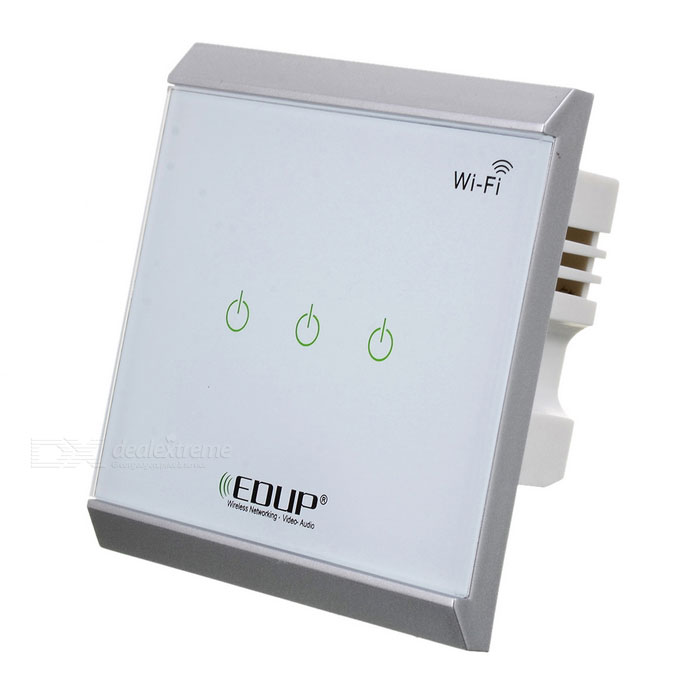
\includegraphics[width=0.5\textwidth]{Figures/edup_light}
\caption{Edup Light Switch}
\label{edup_light_imp}
\end{figure}



\subsection{Bluetooth Beacon}

We require a way to determine if a user is near a certain point in the building such as the office.

From the alternatives seen in Section~\ref{ocupacy_detection}, we  determined that \ac{BLE} beacons are an option to achieve room base location in a building.

There are many kinds of devices capable of emitting \ac{BLE} packets: android devices( available in version 5.0), some microcontrolers and commercial beacon products.

We decided to use a Estimote beacon, the reason it was chosen was because we had one extra around. This beacon also has the advantage of providing temperature readings if needed. Since it is portable we can position it anywhere in the room, enabling better coverage.


\section{Software Architecture}


\begin{figure}[H]
\centering
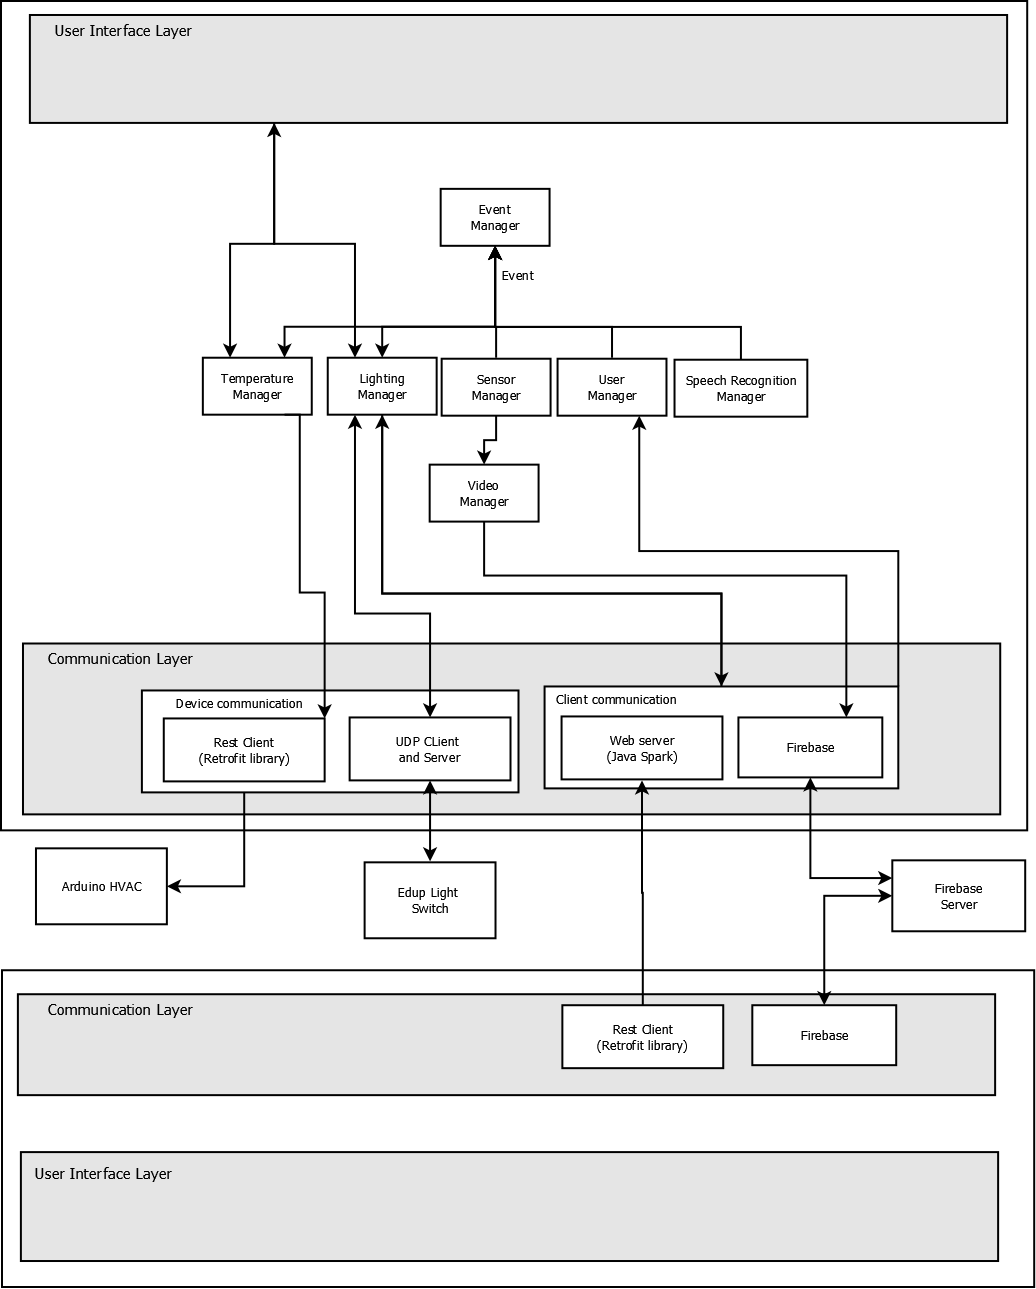
\includegraphics[width=1\textwidth]{Figures/software_dia}
\caption{Software architecture.}
\label{imp:software}
\end{figure}


Our solution is divided into two separate Android applications, the HUB and the USER apps. Both apps work side by side in order to achieve the following functions: user detection, control over \ac{HVAC} and lighting systems, task automation and finally video monitoring \& security. These functions are the building blocks which enables our solutions to achieve building automation, increase user comfort and security monitoring.


\subsection{User Detection}\label{user_detection_imp}

One energy wasting problem is having lighting and \ac{HVAC} systems turned on when no one is present.


In order for our system to take informed actions to cut wasted energy consumption we need to know the location of users inside the building.


The location detection is handled solely by the USER APP. After it confirms the user is inside the building or office it communicates with the HUB. The HUB on the other hand has a timeout system. When a user fails to communicate for a certain amount of time, we presumed he is outside the office or building.

\mbox{}\\
\textbf{In the building}

The building location detection consists in scanning the available \ac{WiFi} networks and checking if the \ac{MAC address} of the \ac{AP} matches a list of pre-scanned \ac{AP}s. This list of pre-scanned \ac{AP}s is sent to the USER APP by the HUB.  

Scanning for \ac{AP}s is battery draining and should be kept to a minimum. We could scan every minute all the time, but decided to start scanning only when a phone connectivity changed. For example when a user enters a building his phone connects to a known \ac{WiFi} network, we use this event to start scanning if the user is inside the target building.


This solution ensures the scanning would start when the user is near a known \ac{WiFi} network. One problem with just this solution is the scanning would go on forever even if we left the office and went home. If after the first five scans (5 minutes), no matching \ac{MAC address} is found the scanning is disabled until a new connectivity change happens. 


In order to implement the above solution we use an Android BroadcastReceiver to be informed when the phone changes connectivity. Then we use an AlarmManager to trigger the scanning code every minute.

\mbox{}\\
\textbf{In the office}

There is an Estimote beacon in the office broadcasting a \ac{BLE} signal. The USER APP is scanning for these signals and when one is found it checks if the namespace in the beacon package matches the known office namespace. After a correct match is found the USER APP informs the HUB the user is near the office.

The \ac{BLE} signal scanning runs for 1 second and then waits 4 seconds before resuming the scan. This means the USER APP notifies the HUB at most every 5 seconds when it is in the proximity of the office.

While Bluetooth LE is a lower-energy system than traditional Bluetooth, scanning is still a fairly power-intensive operation. If our app constantly scans for beacons, it drains the battery at a similar rate as the phone cellular radio. To limit the battery drain we only start scanning when the user is in the building and stop after he leaves.

\subsection{Lighting control}\label{light_imp}


The lights in the room are controlled by the Edup Light Switch, the switch must be connected to a WiFi network and automatically establishes a connection to Edup servers to enable remote control over the switch.

To control the light switch we must send a byte array with the data shown in Figure~\ref{edup_imp}.
The message starts and ends with specific hex strings, the middle part of the message seems to always start with "ZH03", followed by the light switch id then a 1 and finally the lights state we want to change. For example if the ending part of the middle message is "101" then the first and last lights are turned on, and the middle one turned off.

Since there is a physical light switch interface we must update our application status if a button is pressed outside our app.
The Edup Light Switch sends a \ac{UDP} multicast message when the lights are changed. We implemented \ac{UDP} server, when any message is received the content is verified in order to determine if it is a Edup Light switch message. The message must start with "7e7e000d0002" and end with "7f7f". The middle text is "1101", the first character is always the same and the three other represent the current status of the lights.

There were some difficulties since there is no official API. In order to understand how the light switch worked, we used Wireshark to sniff the traffic connection and tried to replicate the messages.

One other problem arises when we quickly turned on/off all the lights in quick succession. When we turn off the first light at the app the light switch sends the multicast message to notify the network, but if we have already turned off the second light then by the time the \ac{UDP} multicast message arrives the state is already different and some lights my turn on back again. To fix this problem when a light is pressed in the app we ignore any \ac{UDP} message for 3 seconds.


\begin{figure}[h]
\centering
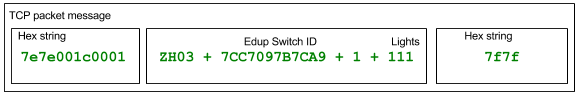
\includegraphics[width=0.8\textwidth]{Figures/Edup_imp}
\caption{Edup packet to set the light state.}
\label{edup_imp}
\end{figure}



\subsection{HVAC control}

Our HVAC solution uses an Arduino with a webserver to control a relay in order to interface with the existing HVAC system.

To get temperature readings from the Arduino \ac{HVAC} and we do a \ac{HTTP}  GET request to the Arduino device \ac{IP} address at the "/data" endpoint. We receive a \ac{JSON} message containing the temperature and humidity. There is a discovery mechanism to setup the Arduino IP it will be mentioned in detail later.

To turn on/off the \ac{HVAC} we send a POST request containing a \ac{JSON} message containing the relay channels we want to turn on/off. In Figure~\ref{arduino_post_imp} the channel configuration is shown. If we want cold air   and slow speed we set the "ch1" to 1 and "ch3" to 1, the other channels must be set o zero ,the \ac{HVAC} starts sending cold air.


\begin{figure}[h]
\centering
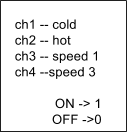
\includegraphics[width=0.3\textwidth]{Figures/temperature_post_imp}
\caption{Arduino HVAC configuration.}
\label{arduino_post_imp}
\end{figure}




\subsection{Automation}

One of the goals of this project is enabling the automation of lighting and \ac{HVAC}. A simple example of an automation task is turning off the lights when no occupant is inside the office.
With our project we aimed to give the user high control and flexibility over the automation process. We allow the user to create chains of simple conditional statements, called "recipes", which are triggered based on events relative to the office.


The recipes contain a list of triggers and actions. A recipe can have one or multiple triggers, when there are multiple triggers we use the logical AND operator, all the triggers must be true in order for the recipe to be triggered.

There are seven triggers available:

\begin{itemize}
  \item \textbf{Temperature:} This trigger allows the user to trigger an action when the office temperature is bellow or above a value specified.
  \item \textbf{Motion:} The motion sensor is triggered when something changes in the field of view of the Hub or no movement detected in X seconds.
  \item \textbf{Speech:} Say the keyword "my assistant" and after the beep you say the phrase specified in the trigger.  
  \item \textbf{Time:} The timer trigger allows the user to run certain actions at a specific time(Scheduler).  
  \item \textbf{User location:} Allows the user to choose from a list of different scenarios ("User is inside office", "User is inside building", "User leaves office", "User leaves building", "User arrives at office", "No user inside building", "No user inside office" and "User arrives at building").
  \item \textbf{Light sensor:} The light sensor triggers an action if the light level is bellow or above the value specified.
  \item \textbf{Light state:} This trigger allows the user to trigger an action when the lights are in specific state.
  
\end{itemize}

The actions available are:

\begin{itemize}
  \item \textbf{Light:} Sets the state of the lights.
  \item \textbf{Temperature:} Changes the target temperature and turns on the HVAC if needed.
  \item \textbf{Speech:} This action uses the speakers to say the text specified (text to speech).
\end{itemize}


In order to show the flexibility of our solution we created the following example recipes:
\begin{itemize}
  \item If a user is in the office and the temperature is above 25ºC then we turn on the cooling.
  \item If no user is inside the office then turn off all the lights and the HVAC.
  \item If the user says "turn on lights" then turn on all the lights.
  \item if the user location status is "user arrives at office", then say "Welcome back".
 
\end{itemize}



\subsection{Communication}

Our solutions has several devices that need to communicate with each other as well as external services.
The HUB needs to communicate with the client, Arduino and light switch. 

Our first approach was to implement both a \ac{REST} server and client in the HUB, the server allowed the USER APP to use an API to control the HUB. The \ac{REST} client allowed the HUB to communicate with external services such as getting weather forecast information or controlling the Arduino.
Latter we decided to also include Google Firebase Database as a communication channel between the HUB and USER APP.


\mbox{}\\
\textbf{Rest server}

We implemented the server using a java SPARK 1.1.2 running at port 5002. The server is launched using a background service running in separate thread.

The server exposes the following Rest API: 

\begin{itemize}
  \item \textbf{GET /register:} Returns the HUB UUID, description and name.
  \item \textbf{POST /register:} Receives the name, email and UUID of a new user. Returns a status true/false depending if the registration was successful.
  \item \textbf{POST /location} Receives an UserLocation object, Figure~\ref{user_location_class}.
  \item \textbf{POST /make-changes:} Receives the temperature value we want "targetTemperature", and receives an boolean array representing the lights we want to change "lightsState";
   \item \textbf{GET /status:} Returns the current temperature and a boolean array representing the lights.
   \item \textbf{GET /alive:} Returns a status "true" signifying the server is running.
\end{itemize}

\begin{figure}[h]
\centering
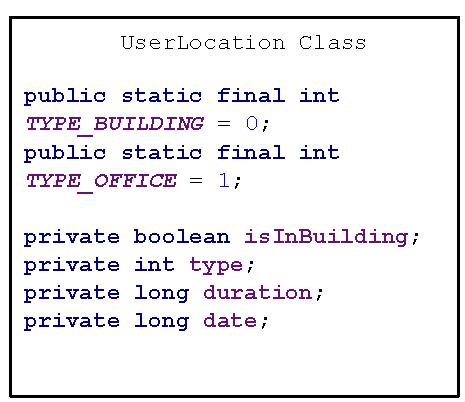
\includegraphics[width=0.4\textwidth]{Figures/userlocation_class}
\caption{UserLocation Class parameters.}
\label{user_location_class}
\end{figure}

Current implementation of SPARK Framework uses JAVA 8, since Android is compatible with JAVA 7 and partially with JAVA 8 we had to use and older version of the SPARK server that runs JAVA 7.  

\mbox{}\\
\textbf{Rest client}

The Rest client allows our apps to initiate communication with a server, it is used by the USER APP to interact with the HUB server and used by the HUB to communicate with the Arduino and Weather forecast API.

We decided to use the Retrofit Android library as our Rest client, this library is one of the most popular Rest client libraries used by developers due to performance and extensibility.



\mbox{}\\
\textbf{Firebase}

Originally the plan was to only use the web server, but in our building we can't run web servers in the WiFi network. When we tried to contact the HUB it did not receive any request, then we changed to a private wireless network it all worked normally.

The solution we found was Google Firebase, it is a platform that offers multiple services. We use two services, the real-time database and the storage.
We use their real-time database to synchronize application data across clients and store it on Firebase's cloud. Using an Android library developed by them we can store JAVA objects directly to the database. The storage service is used to upload the recorded videos and live preview images, captured by the security system.

Firebase solves us two problems, one is users can access our solution from home and access the live camera, Firebase is used as a middle man to communicate. The second problem it fixed was user detection, since our building is big, the private network where the tablet is connected can't be access in most of the building. A user entering the building could not communicate with our HUB and notify of it's presence since they were in different networks, we use Firebase to add our location messages that are then received by the HUB and building user detection is achieved.

We ended having two ways to communicate with the HUB APP, each has some strong and weak points. 

The negative points with Firebase are it requires internet to work so we had to keep the web server in order for our solution to work inside the office even when no internet connectivity was present. One other problem is the free tear only allows 100 simultaneous connections, which means there can only be a maximum of 100 users and HUB devices connect at each moment.

One weak point of the web server is it's response time varies a lot, some times just a few milliseconds up to a few seconds for simple static content. The server is running in a separate thread but while the APP is in the foreground the response times increase a bit.



\mbox{}\\
\textbf{Edup Light Switch Communication}

Communication with the Edup Light Switch required the use of TCP sockets to give commands and an UDP server to listen to changes. The communication with the light switch was previously explained in section ~\ref{light_imp}.



\subsection{Security - Motion detection, video recording, Live view}

With our office being like an extension of our home we felt the need to have some sort of video surveillance system. We created a system capable of detecting if a object is moving inside the office, identify if a user is inside the office and if not then send a notification to the user and record a small video.


\mbox{}\\
\textbf{Motion detection}

The motion detection works by comparing two camera frames. If a percentage of pixels are different we assume motion has happened. Both the percentage of different pixels and the detection period are configurable using the \ac{UI}.

The camera frames are received by accessing the bitmap of the TextureView where the camera picture is shown. We had to use the bitmap from the view and not a camera callback because when video is recording Android does not trigger the camera callback.

In order for a camera frame pixel to be considered different the RGB value of the pixel must be more than 50.


\mbox{}\\
\textbf{Video recording}

When motion is detected and no user is inside the office we record 30 seconds videos. These videos are uploaded and stored to Firebase servers, where the user can latter watch them using the user app.

The videos don't have any audio because Android does not allow the audio to be shared between the speech recognizer and the video recorder at the same time.


\mbox{}\\
\textbf{Live Camera}

We can watch in real time pictures from the office camera. When the user is using the user app live camera functionality, the Hub saves a camera frame every second to Firebase server. We have seen a minimum delay of 4 seconds between the live pictures and the time they were taken.


\subsection{HUB APP}

\begin{figure}[h]
\centering
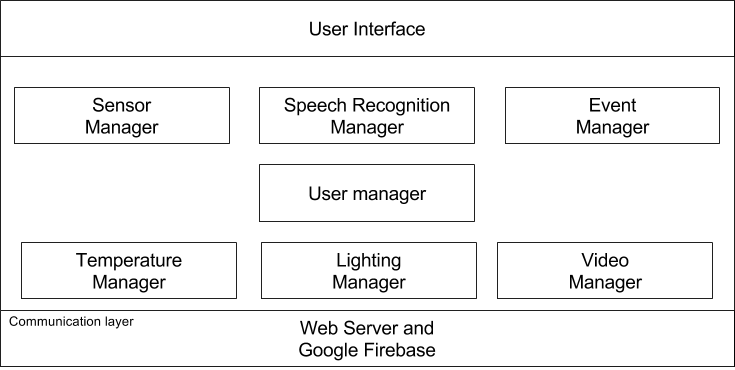
\includegraphics[width=0.7\textwidth]{Figures/software_implementation}
\caption{Software architecture of HUB APP}
\label{software_imp}
\end{figure}


The HUB app is the office controller that interacts with all other devices. The HUB offers a \ac{UI} to manual control the lighting and \ac{HVAC} systems, automation rules and settings. In terms of business logic we implemented a set of managers responsible for different operational requirements of the application.


\subsubsection{Event Manager}

The Event Manager  operates in a publish/subscriber basis. Other managers register their interest in certain events and when whose events happen they are notified. The events can be published to the event manager by any other manager. For example the Sensor Manager can publish a motion detected event, that the video manager is interested.

Currently there are eight different events available:

\begin{itemize}
  \item \textbf{Temperature:} Contain the current temperature and humidity.
  \item \textbf{Motion:} This event contains a boolean to inform if movement is detected, and long value with the time since last movement was detected.
  \item \textbf{Speech:} The phrase of an successful speech recognition.  
  \item \textbf{Time:} If we need to check some task regularly this event is triggered every 2 seconds.  
  \item \textbf{User location:} This event contains the user id, the location type (Office/Building), a boolean to specify if he is in the location or left and finally a boolean to indicate if the user just arrived.
  \item \textbf{Brightness:} The value in Lux of the light sensor.  
  \item \textbf{Light:} The light switch number and it's status. 
  \item \textbf{Change temperature:} The value of temperature we want the thermostat to be at. 
  
\end{itemize}


The Event Manager is also responsible for the automation. When a event is published all the recipes are examined to see if all triggers conditions are fulfilled. When this happens all the actions in that particular recipe are executed.


\subsubsection{Speech Recognition Manager}

The power to control the office/home with our voice is something increasingly popular with the launch of products like Amazon Echo, Google Assistant and Apple Siri. In order to increase the comfort of our users we added speech recognition into the HUB. This allows the user to trigger a recipe with the power of their voice. For example a user siting in his chair could say "turn on the lights" and the office lighting would trigger. 

This manager uses the CMU Sphinx offline keyword speech recognizer, meaning it will detect one word in our case "my assistant". When it detects the keyword it shuts down and we launch Google online speech recognition. We use this other speech recognition because it offer better results, the reason the manager uses two different speech recognizes is because using only Google recognizer has higher bandwidth cost since we would be constantly sending audio. The other reason is privacy, we don't know if Google is going to disclose our audio files to third parties.

When we successfully say the keyword a beep sound is played and Google speech recognizer listens to the rest of the voice command, when the results arrive from Google they are published to the Event manager.

There were several problems with both recognizer, the Sphinx has a lot of false positives for small words, for our current keyword we sometimes need to repeat more than once for it to recognize. This problem can perhaps be attributed to the fact we are not native English speakers. 
Google speech recognizer is plagued with problems since a few version ago, it sometimes will not listen and shutdown after some 100 ms. To try to minimize the problem by run a check every 10 seconds. If both speech recognizes are not running we relaunch Sphinx.

\subsubsection{Sensor Manager}\label{sensor_manager_imp}

The Sensor Manager is responsible for the light sensor and virtual motion sensor.

The light sensor is built in in the tablet. Every 2 seconds the current light level is published to the Event manager. 

Since the tablet does not have a motion sensor, we use the front camera and analyze the frames every second. If the total number of the RGB pixels with threshold above 50 is different we know there was a change in the eye sight of the camera. The percentage of different pixels for a positive detection is user defined, the default is 0.5\%.

A problem that motion detecting cameras have are the false positives specially when there is a windows to the outside. A strong light can trigger the sensor, because of that we designed the sensor to be able to ignore an area of the camera frame. It is possible to specify the area to ignore in the Hub app settings.


\subsubsection{Video Manager}

The Video manager does two jobs, it records 30 seconds videos when no user is present in the office and motion is detected. The other job is offering a live preview of the office, an user can use the user app to watch in real time the office.

The recorded videos don't have any audio because Android does not allow the audio to be shared between the speech recognizer and the video recorder at the same time.

The video manager can be enabled and disabled in the HUB settings for privacy reasons.



\subsubsection{Lighting Manager}

This manager is responsible for turning on/off the room lights and keeping their status updated when a user uses the manual switch. 






\subsubsection{Temperature Manager}\label{temperature_manager_imp}


The Temperature Manager is responsible for keeping an updated weather forecast, keeping an updated temperature reading and turning on/off the Arduino \ac{HVAC}.

The forecast uses Wunderground service API and is used to give information to the user about the current weather conditions.

There are two different configurations to access the temperature in our solution, using an Estimote beacon or the Arduino \ac{HVAC}. 
The beacon sends a Eddystone telemetry packet containing the current temperature, it is intended for situations when we just want to display the temperature.
The Arduino option gives the temperature and humidity and allows us to control the \ac{HVAC} system.


In order to obtain the beacon temperature, it must be configured to the Eddystone-UID primary packet type using the Estimote mobile app. Then the beacon namespace must be set in the Hub app settings.


\subsubsection{User Manager}


The User Manager keeps track of the user location (in building, in office) and is responsible for registering new users.

The location system works in the following simplified manner, it receives two types of location messages from the USER APP, in-building or in-office, there are timeouts in place so in the eventuality that no message is received for a certain amount of time we assume the user has left the office or building. The in-building messages arrive every 60 seconds and in-office every 5 seconds, the timeouts are 120 seconds and 20 seconds respectively.


There are two types of user that can register. Users with the mobile USER APP and users without it. If a user has the app, it just needs to open the app and there is an semi-automatic register process. If the user does not have the app he will receive an email with an QR-Code that will act as an identification card, when the user places the card in front of the HUB camera he is logged on for a certain amount of minutes specified by the user. Since we can't track the user whereabouts without the app, the user will have to manually turn the lights and \ac{HVAC} if he leaves while logged on.



\subsubsection{User interface}


The \ac{UI} of the HUB APP is composed of three main screens. There are a lighting screen, a temperature and general menu that contains several advanced features.

The \textbf{lighting screen}, shown in Figure~\ref{screen_lights} allows the user to control the lighting environment in the room.

The \textbf{temperature screen}, shown in Figure~\ref{screen_temperature} gives visual information about the current weather outside. There is also a virtual thermostat where the user can select the temperature he desires. The thermostat shows a leaf icon when the selected temperature is inside the range of temperature where people are comfortable as described in section~\ref{related:adaptive_heating}. 

There is a \textbf{general menu} that contains the other screens that enable additional features. This menu contains:
\begin{itemize}
  \item \textbf{User registration:} Allows the a person to setup an account in Hub. 
  \item \textbf{Recipe management:} Contains a list of the current recipes in the Hub and allows the user to create, edit, disable/enable and delete them.
  
  \item \textbf{Event history} Shows a list events ordered chronologically. 
  
  \item \textbf{Statistics screen} Shows temperature, lighting and occupation graphics. 
  
  \item \textbf{Settings screen} Allows the user to configure the Hub app.
\end{itemize}



The \textbf{user registration screen} allows the user to register using the user app or an email address.
If the user uses the Android user app, a visual registration token is shown in the form of a QR-Code. The QR-Code contains a temporary id and the IP address of the HUB server. This temporary id is latter needed when the user registers and exists  only to ensure only people inside the office can register and not just anyone that knows the IP address.

In the \textbf{recipe screen}, the user can create new recipes, first the trigger/s is selected, only then can the action/s be picked. In Figures \ref{create_recipe}, \ref{screen_triggers}, \ref{screen_actions} and \ref{screen_completed_recipe} the steps needed to create a recipe are shown, the resulting recipe turns on all the room lights if a user is inside the office and the light level is low. 

The \textbf{settings screen} allows the user to change:
\begin{itemize}
  \item Number of lights.
  \item Edit the Edup light id.
  
  \item Set the motion detection threshold (percentage of different frames for positive detection)
  
  \item The camera detection period, the time between consecutive motion detection.
  
  \item Specify an area in the camera frame where motion is ignored, described in Section \ref{sensor_manager_imp}. 
  
  \item Video recording, enable/disable recording when no user is present and movement is detected.
  
  \item Live preview, allow users to watch the office in real time, using the USER APP.
  
  \item Scan for Arduino/HVAC, as mentioned in Section\ref{temperature_manager_imp} there is discovery mechanism to add the Arduino and control it. We use \ac{SSDP} to discover supported Arduino devices and list the discovered device/s. The user then selects the device specific to his office.
  For an Arduino device to be shown, they have to been programmed to be discoverable using the protocol and have the search target equal to "schemas-basa-pt:service:climate:1".
  
  \item Estimote beacon namespace, the id of the estimote beacon we want to get the temperature reading.
  
  \item Building location, the list of \ac{MAC address} separated by comma of the building. Used by the User app to determine if they are in the correct building.
  
  \item Room location, the list of Estimote beacon namespace associated to the office.
  
  
  \item Enable Kiosk mode, this mode disables the home and power button of the Android device. It prevents a user from closing the app. 
    
  
\end{itemize}

%\centerline{
% 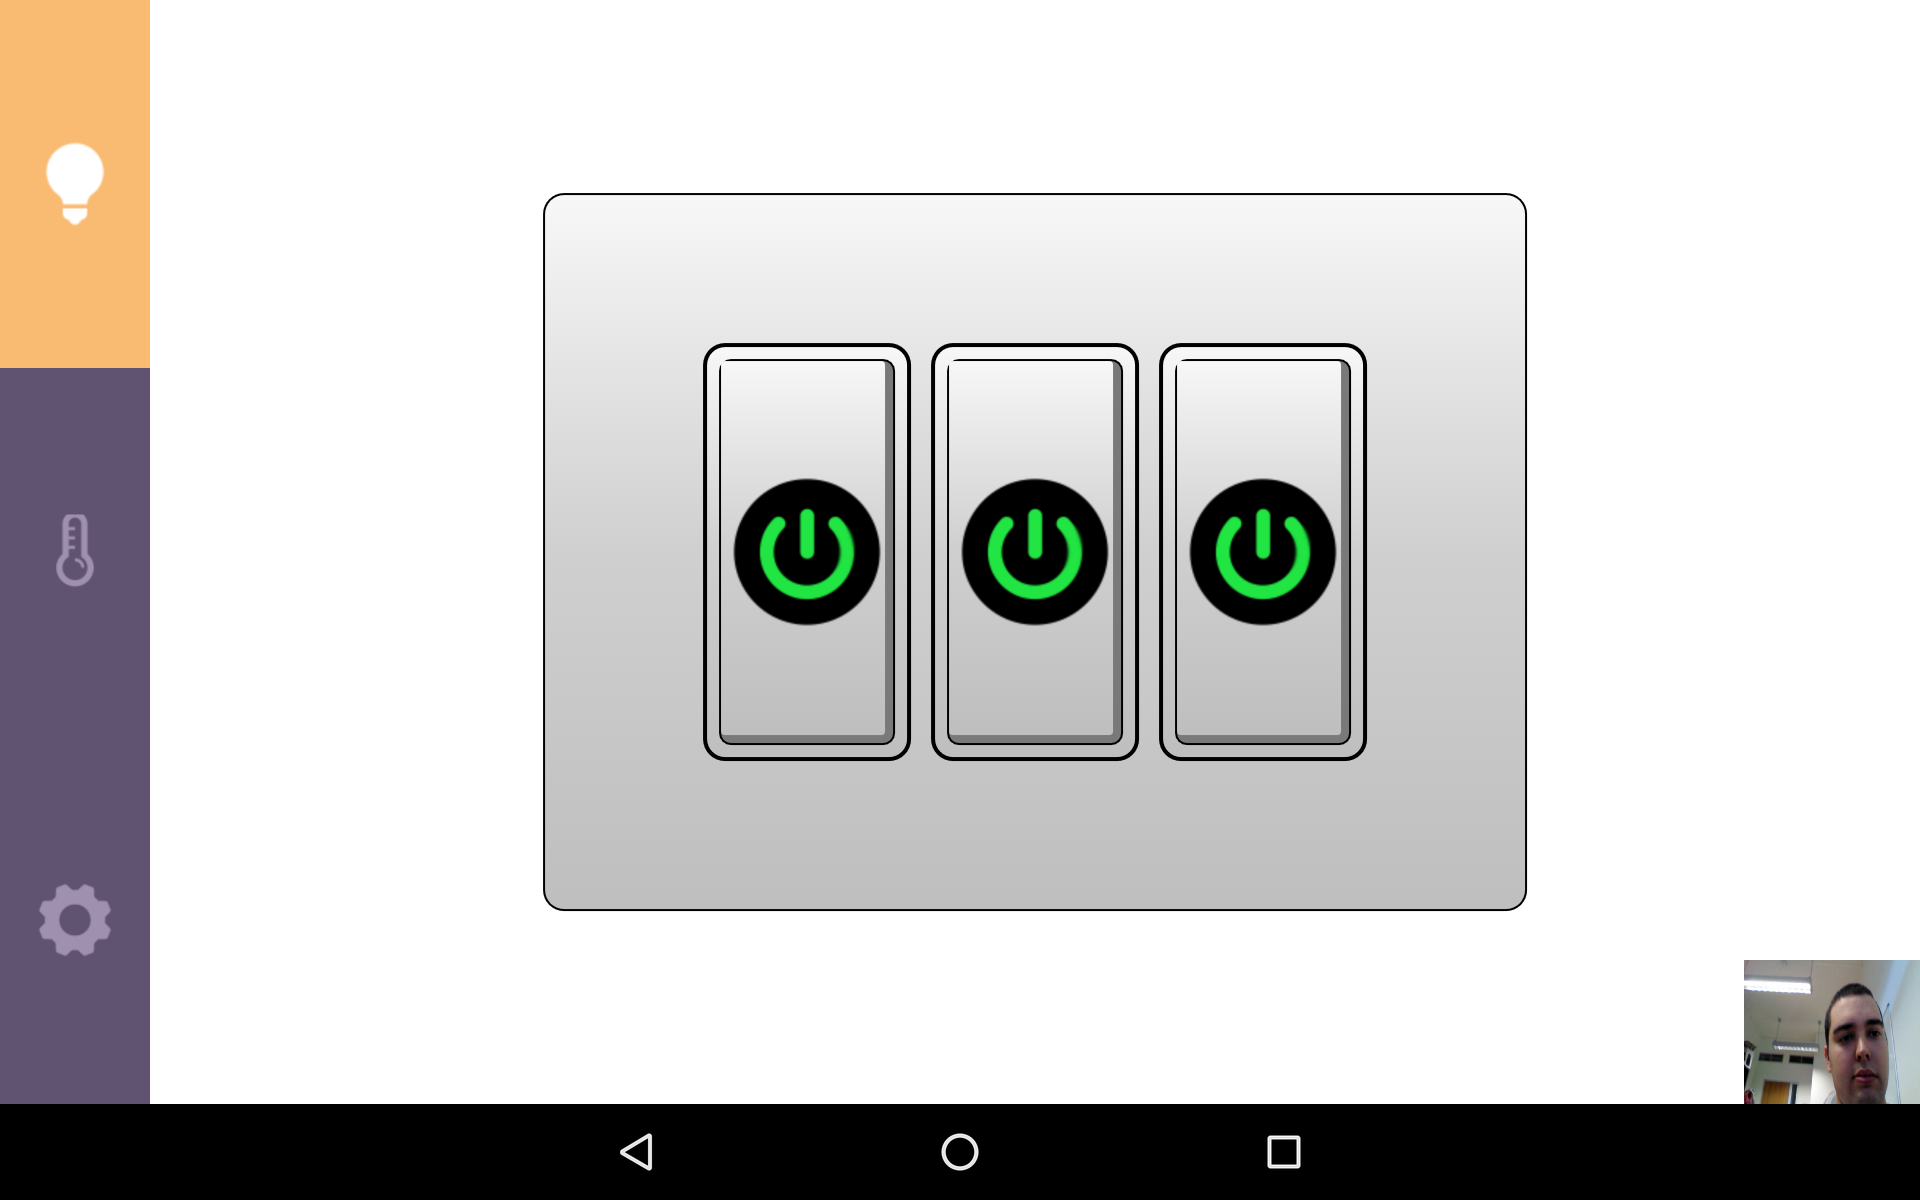
\includegraphics[width=90mm]{Figures/screen_lights}
%}
%
%\centerline{
% 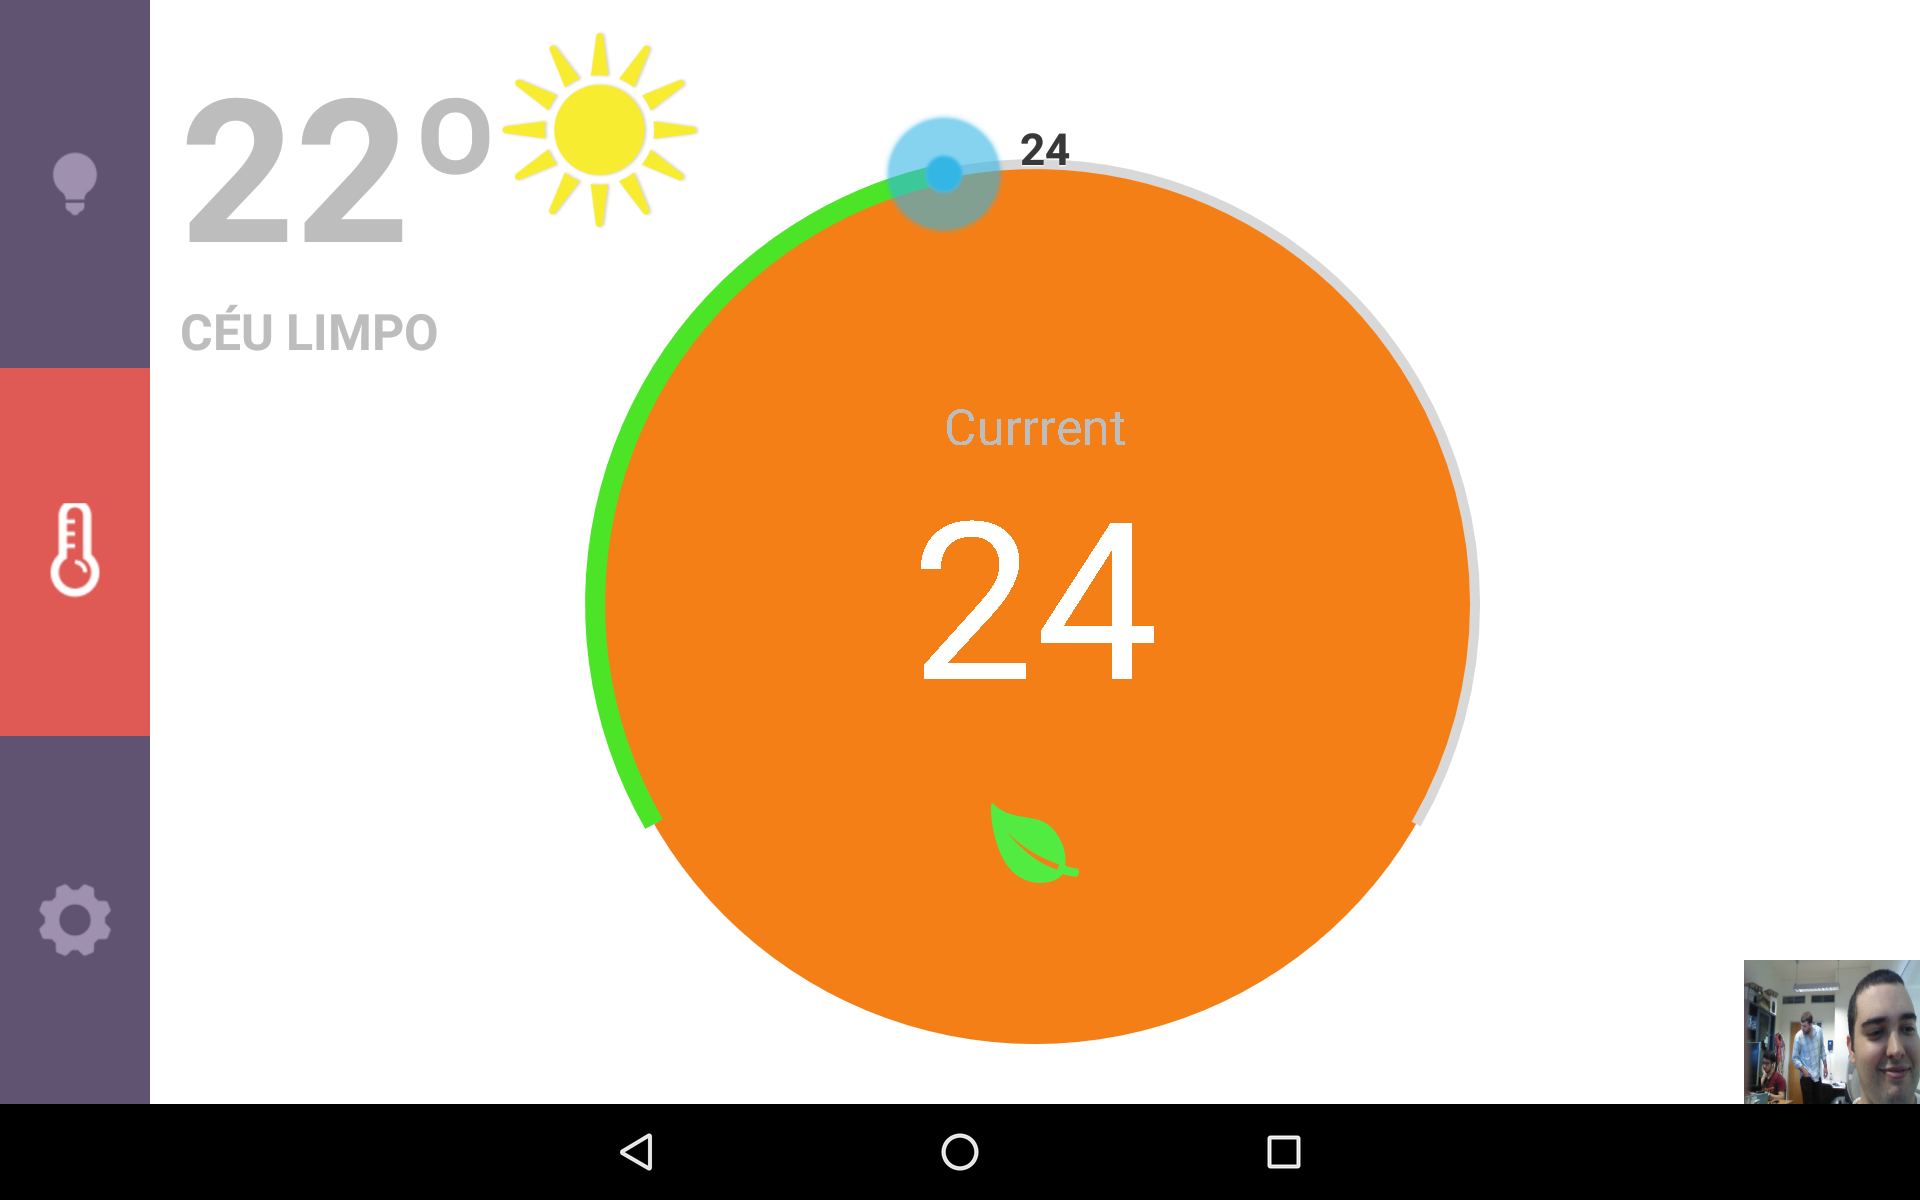
\includegraphics[width=90mm]{Figures/screen_temperature}
%}


\begin{figure}[H]
\centering
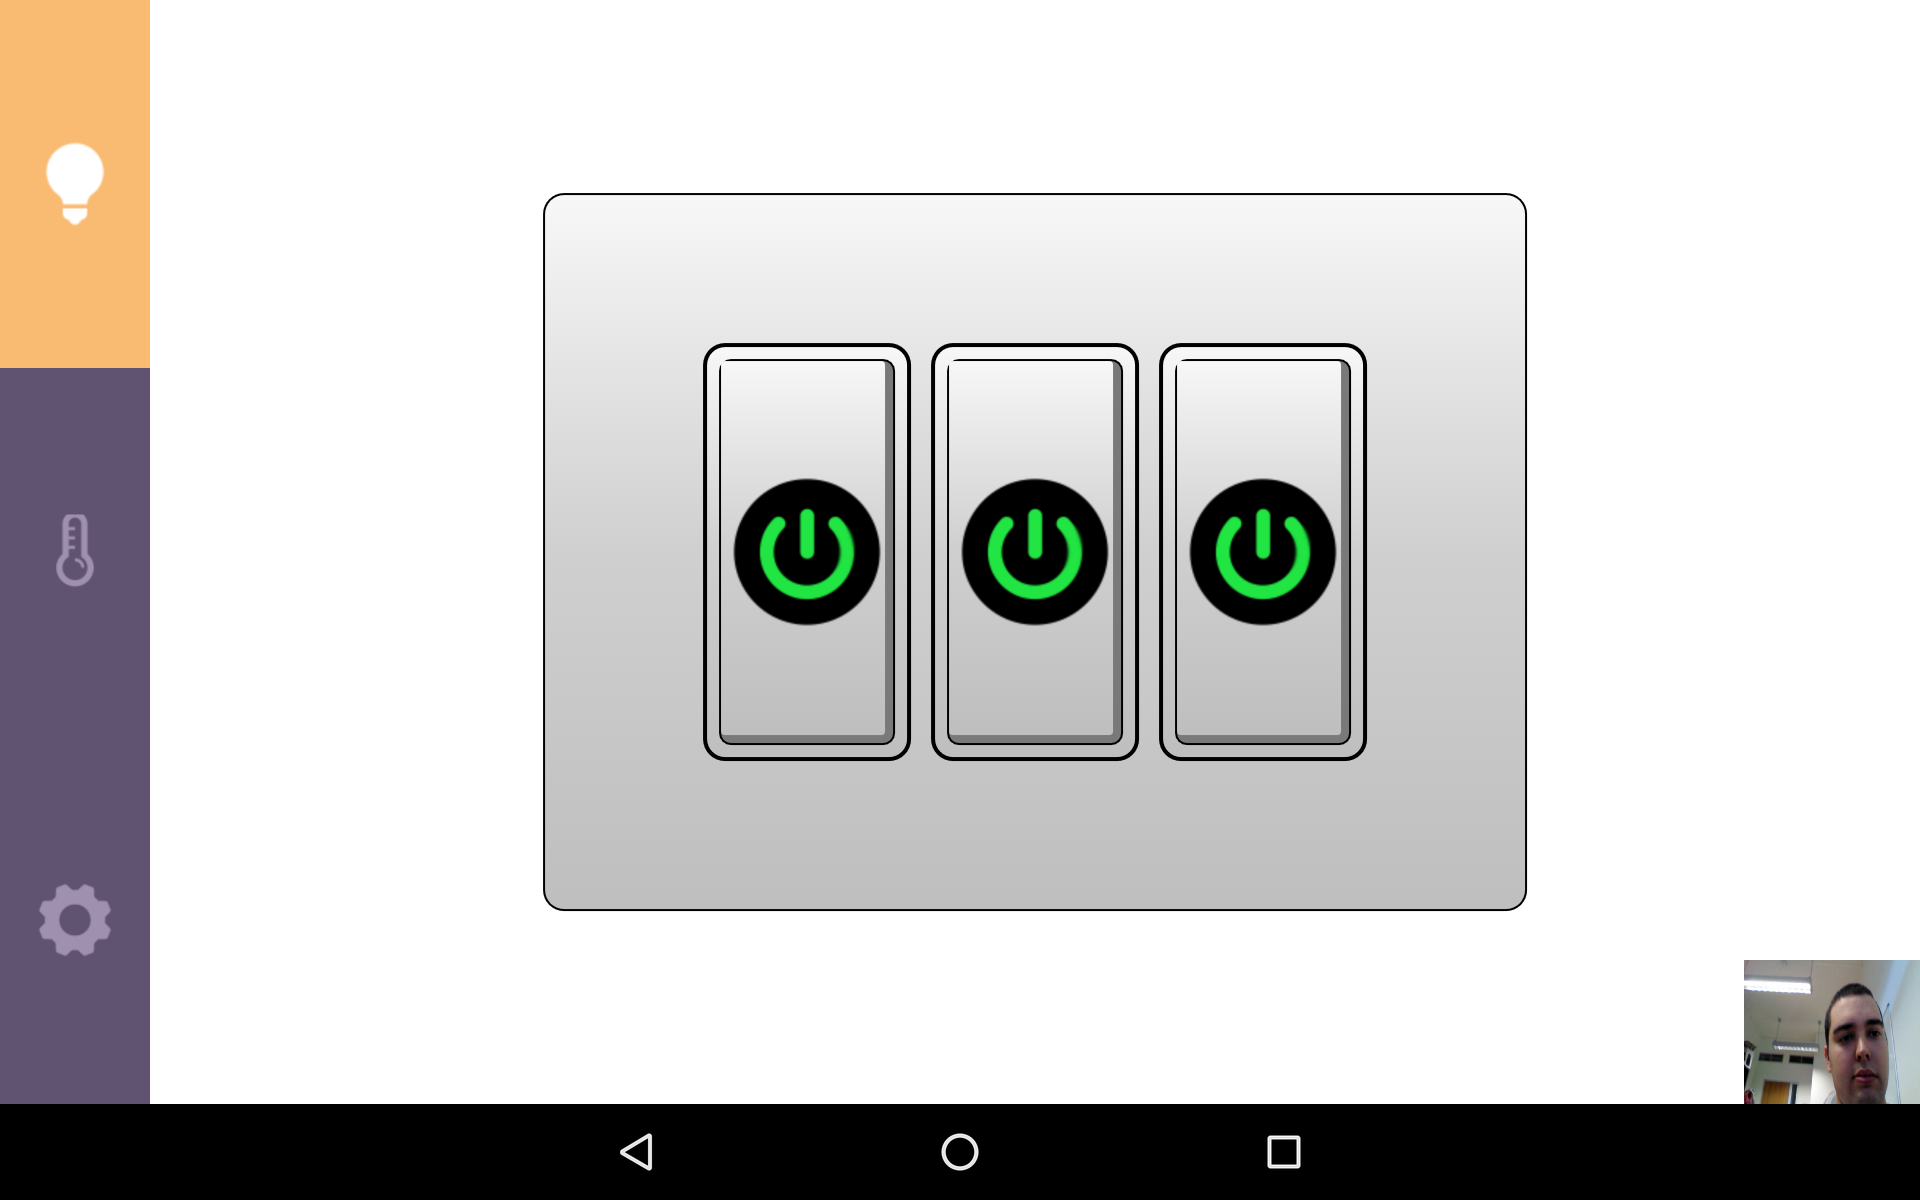
\includegraphics[width=0.6\textwidth]{Figures/screen_lights}
\caption{Light fragment.}
\label{screen_lights}
\end{figure}


\begin{figure}[H]
\centering
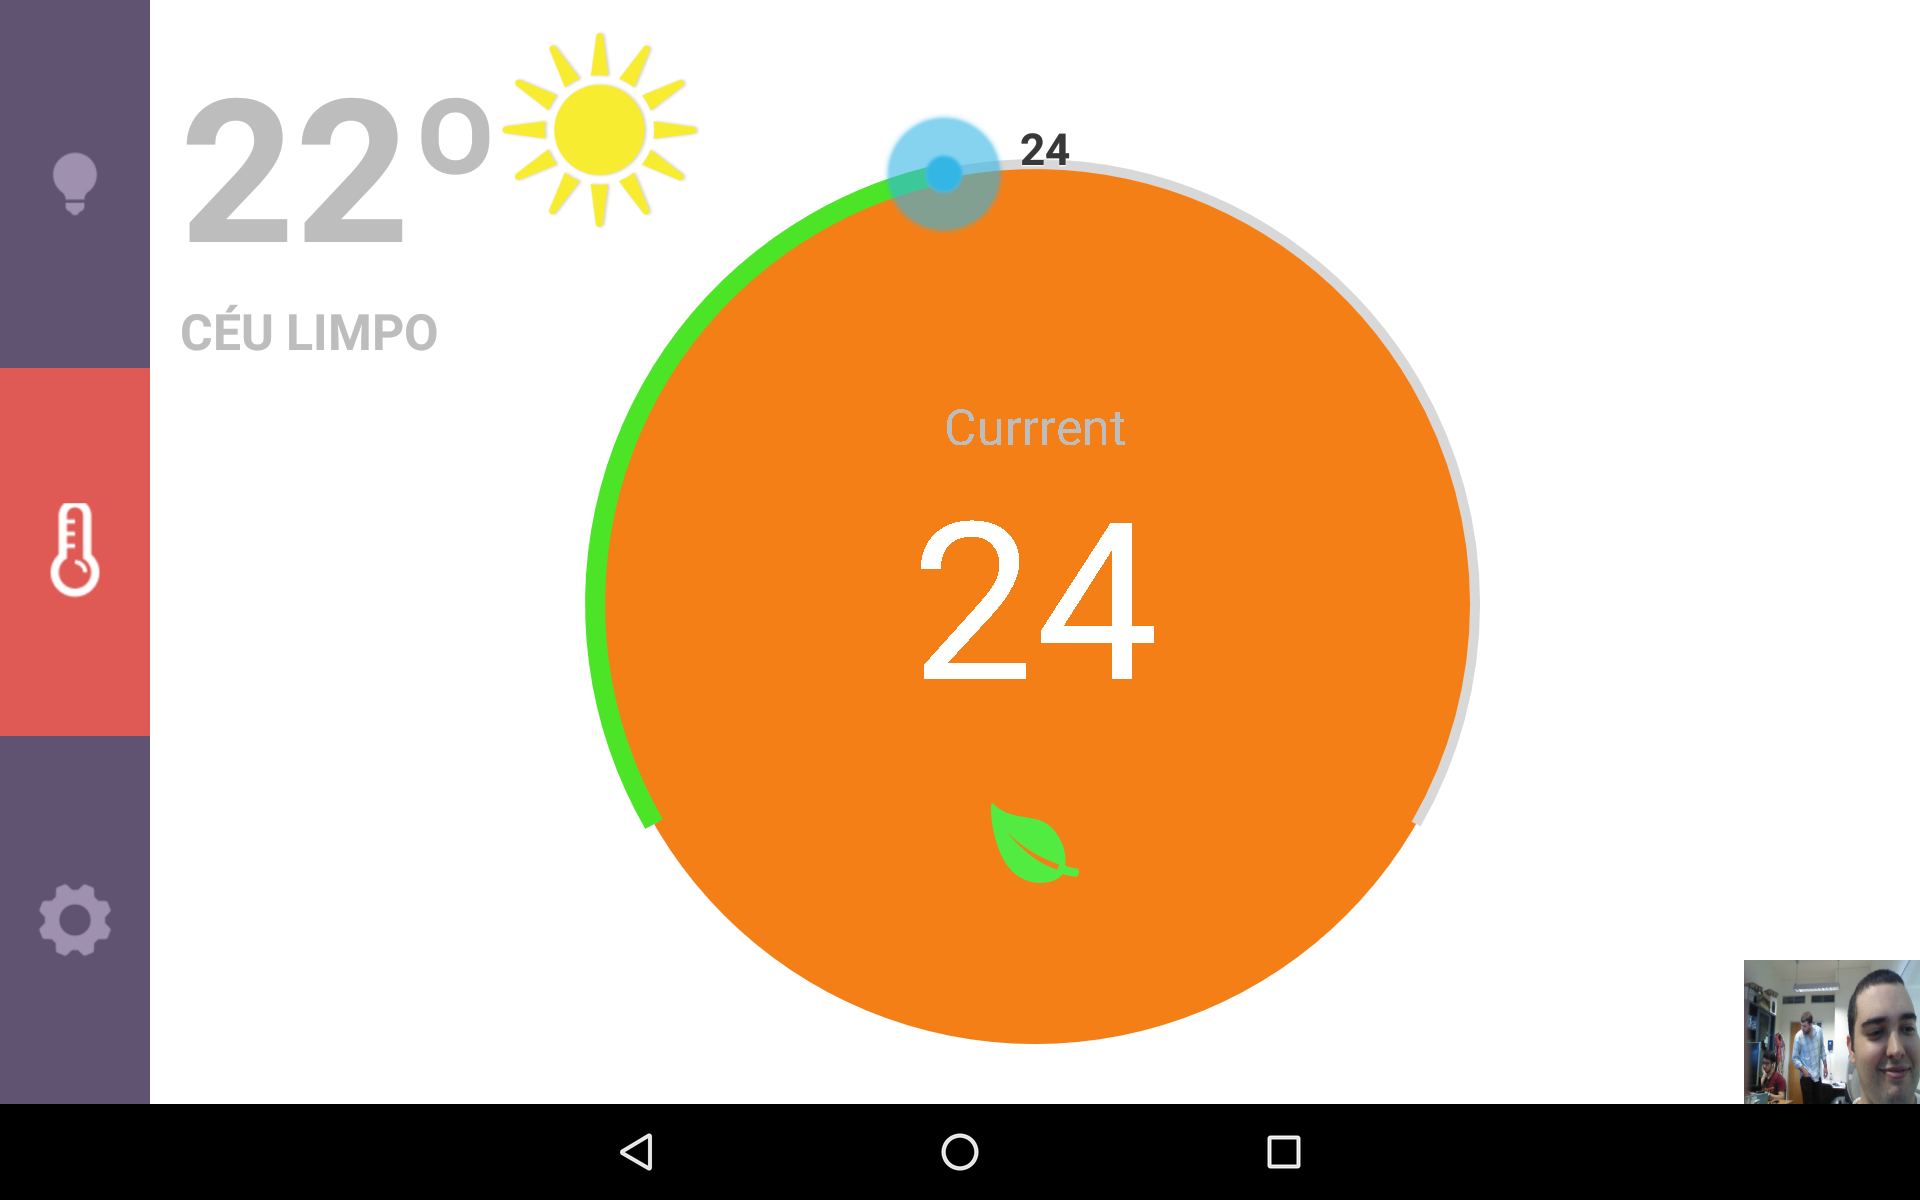
\includegraphics[width=0.6\textwidth]{Figures/screen_temperature}
\caption{Temperature fragment.}
\label{screen_temperature}
\end{figure}



\begin{figure}[H]
\centering
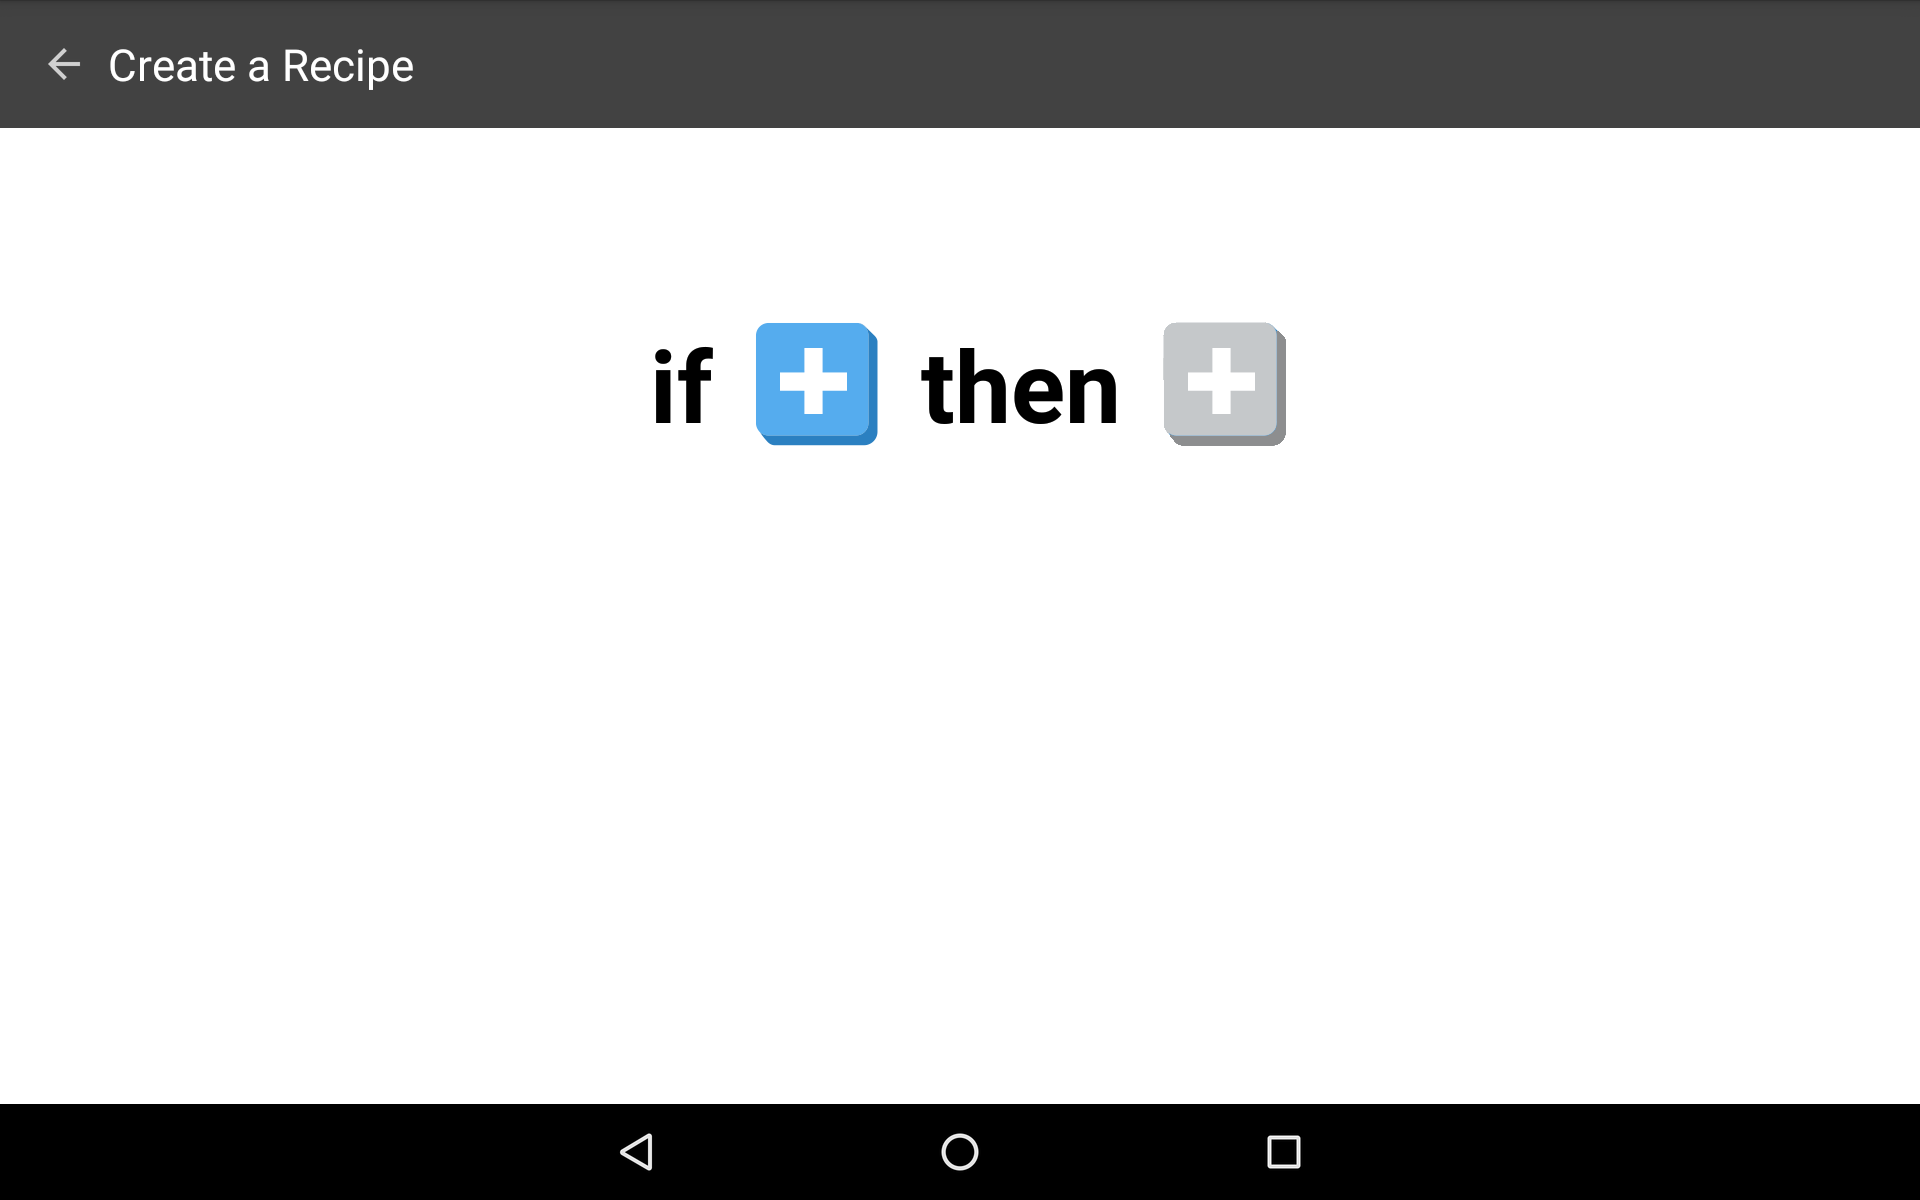
\includegraphics[width=0.6\textwidth]{Figures/create_recipe}
\caption{Create recipe fragment.}
\label{create_recipe}
\end{figure}

\begin{figure}[H]
\centering
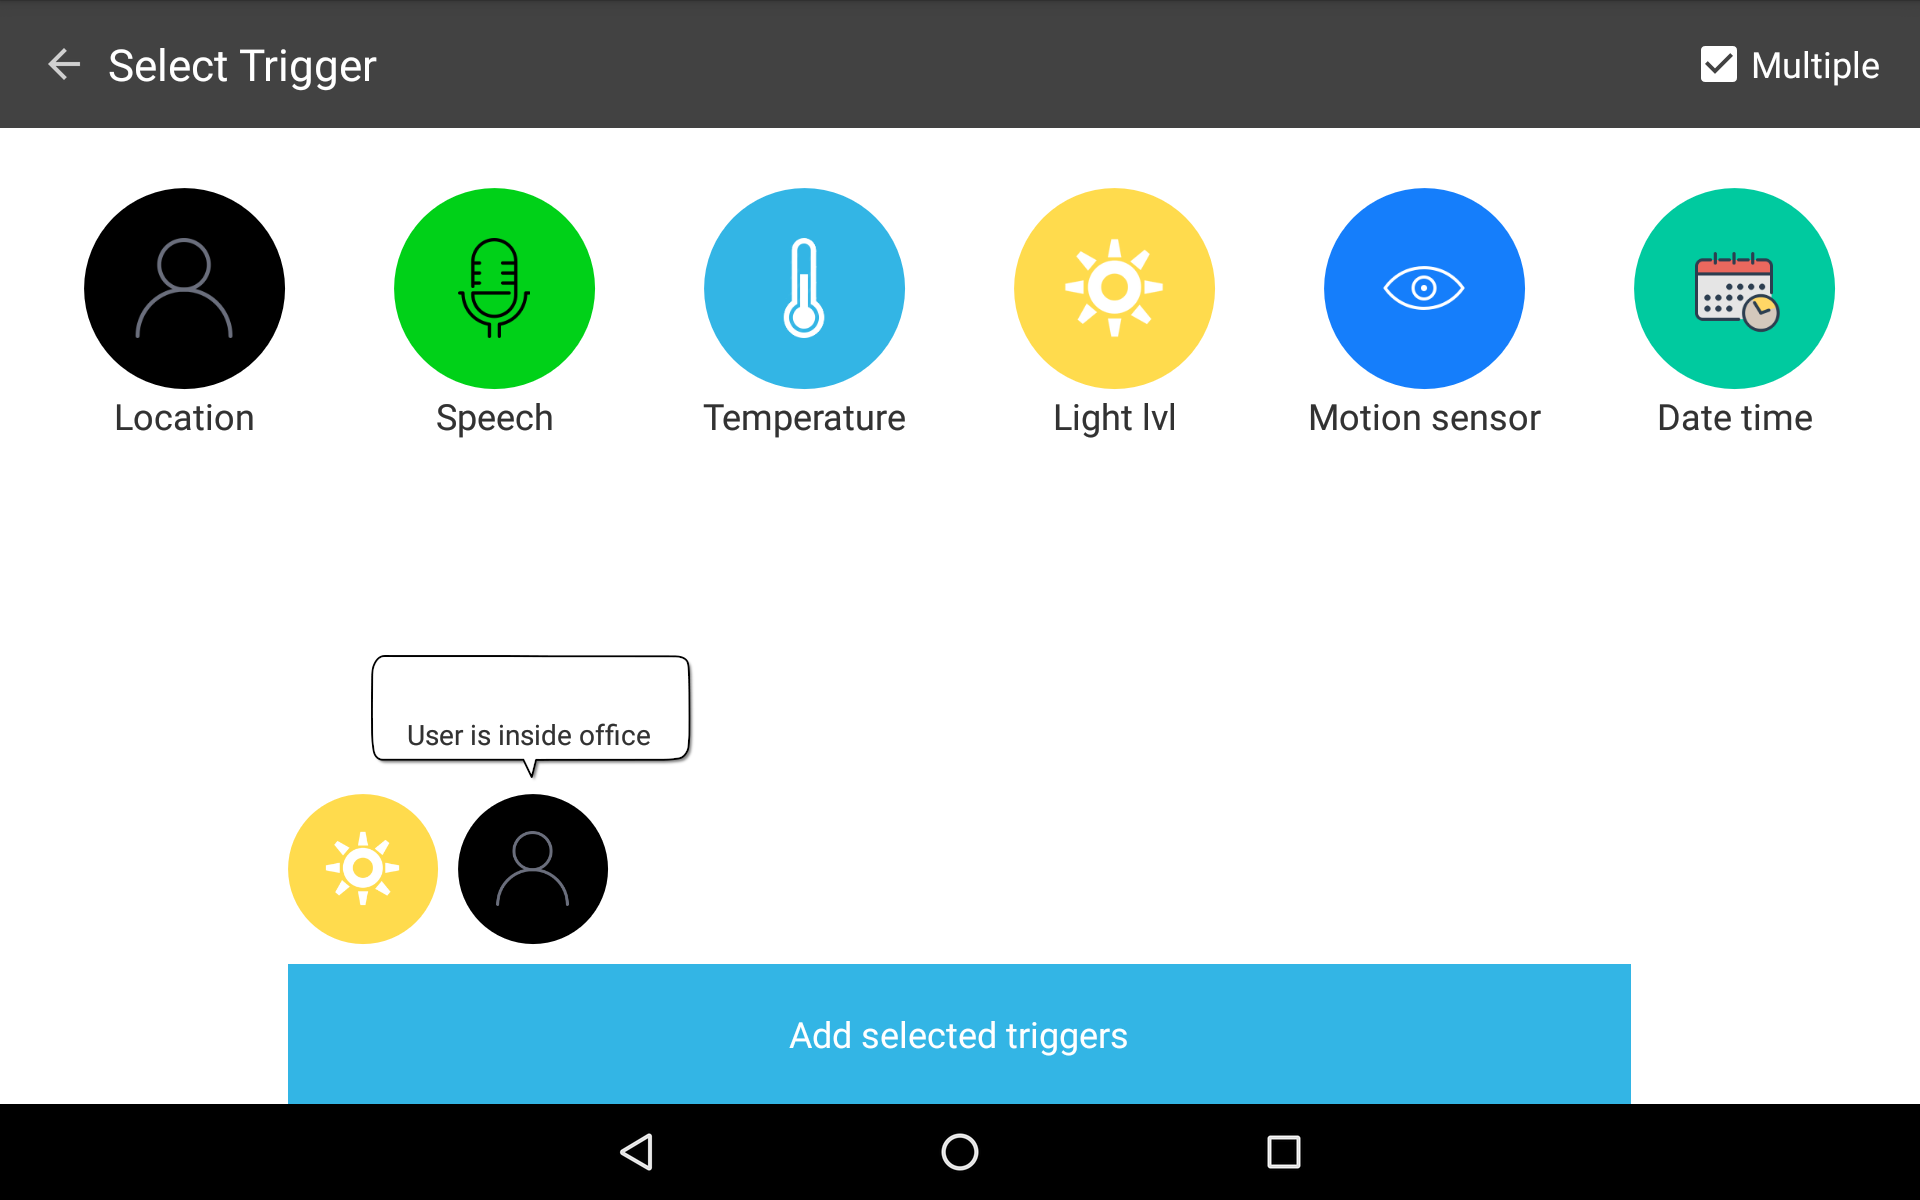
\includegraphics[width=0.6\textwidth]{Figures/screen_trigger}
\caption{Add trigger fragment.}
\label{screen_triggers}
\end{figure}

\begin{figure}[H]
\centering
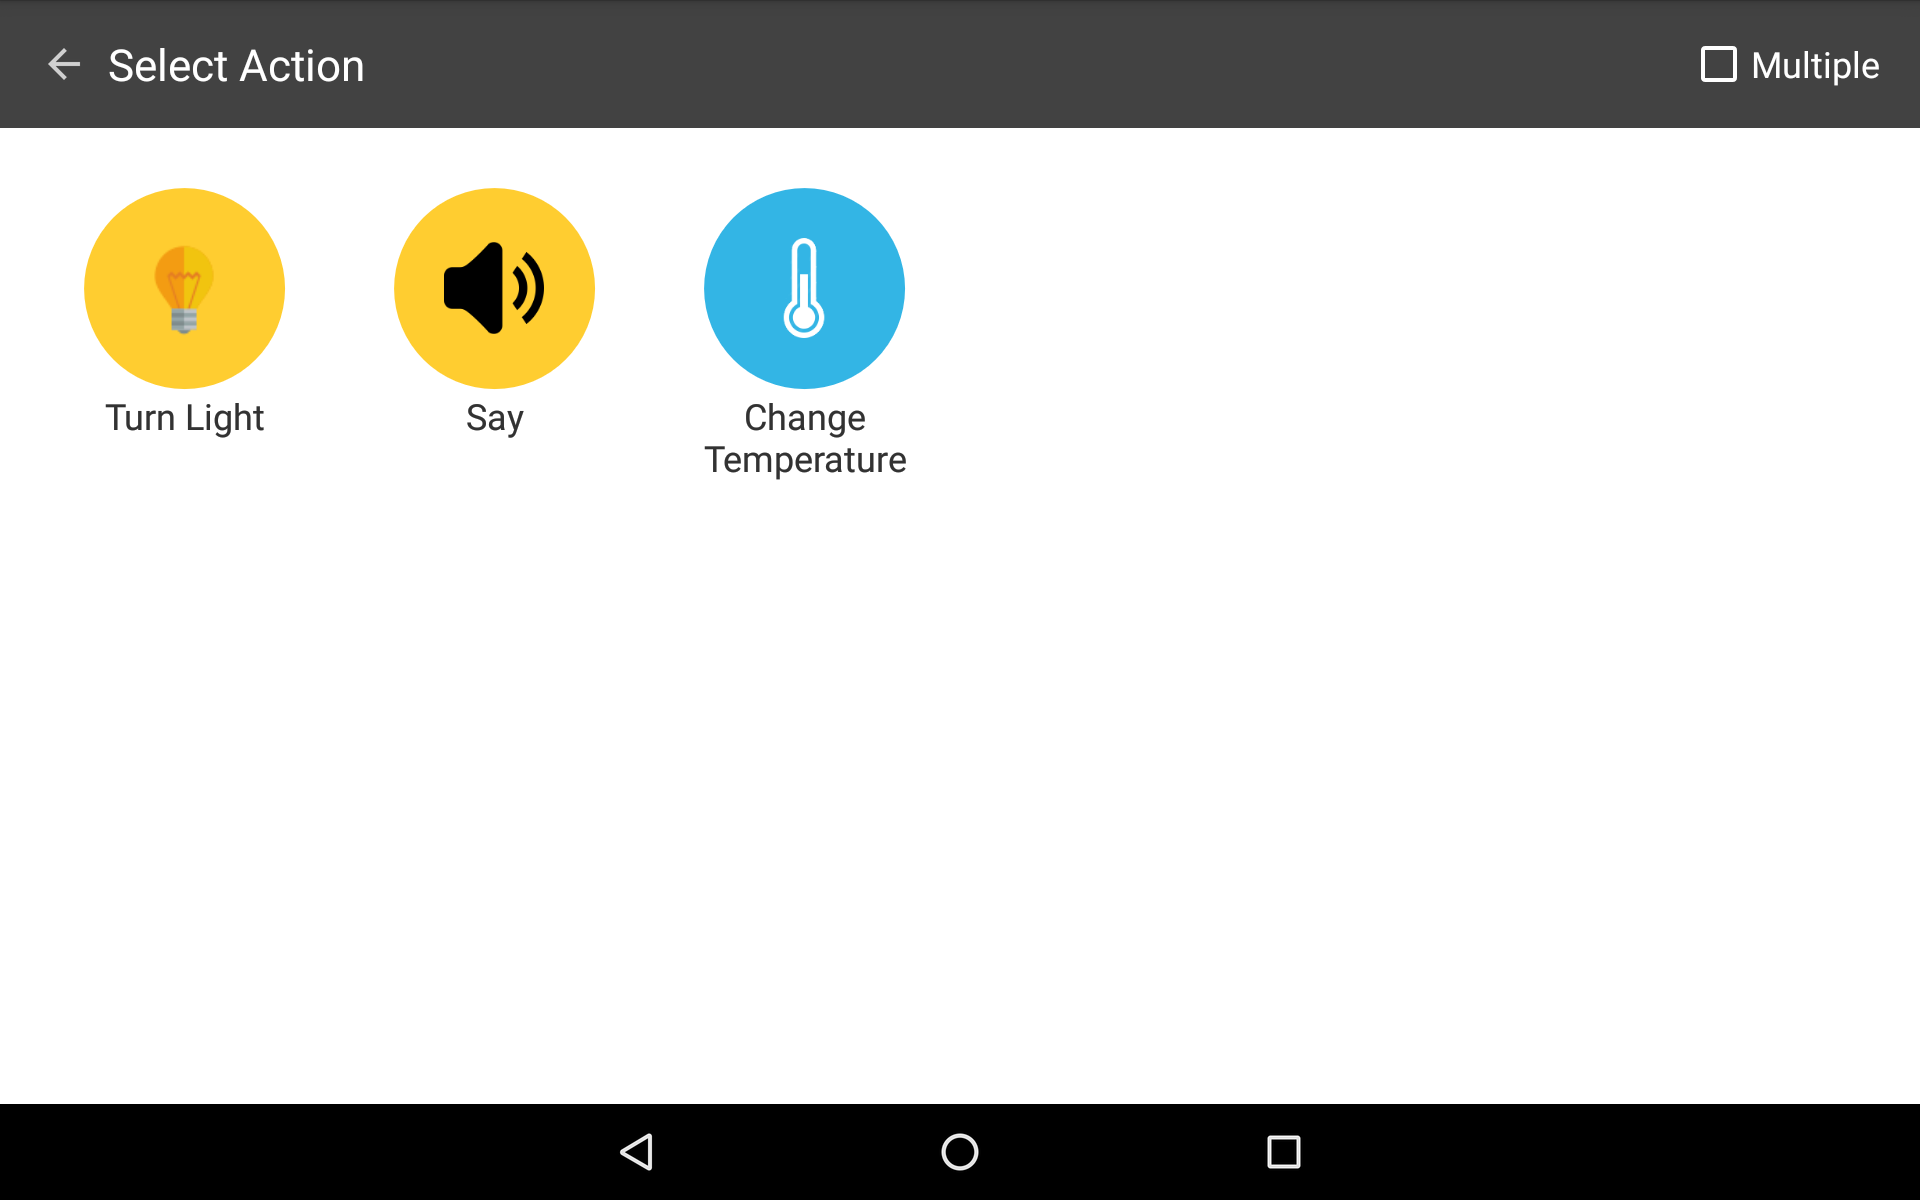
\includegraphics[width=0.6\textwidth]{Figures/screen_actions}
\caption{Select action fragment.}
\label{screen_actions}
\end{figure}

\begin{figure}[H]
\centering
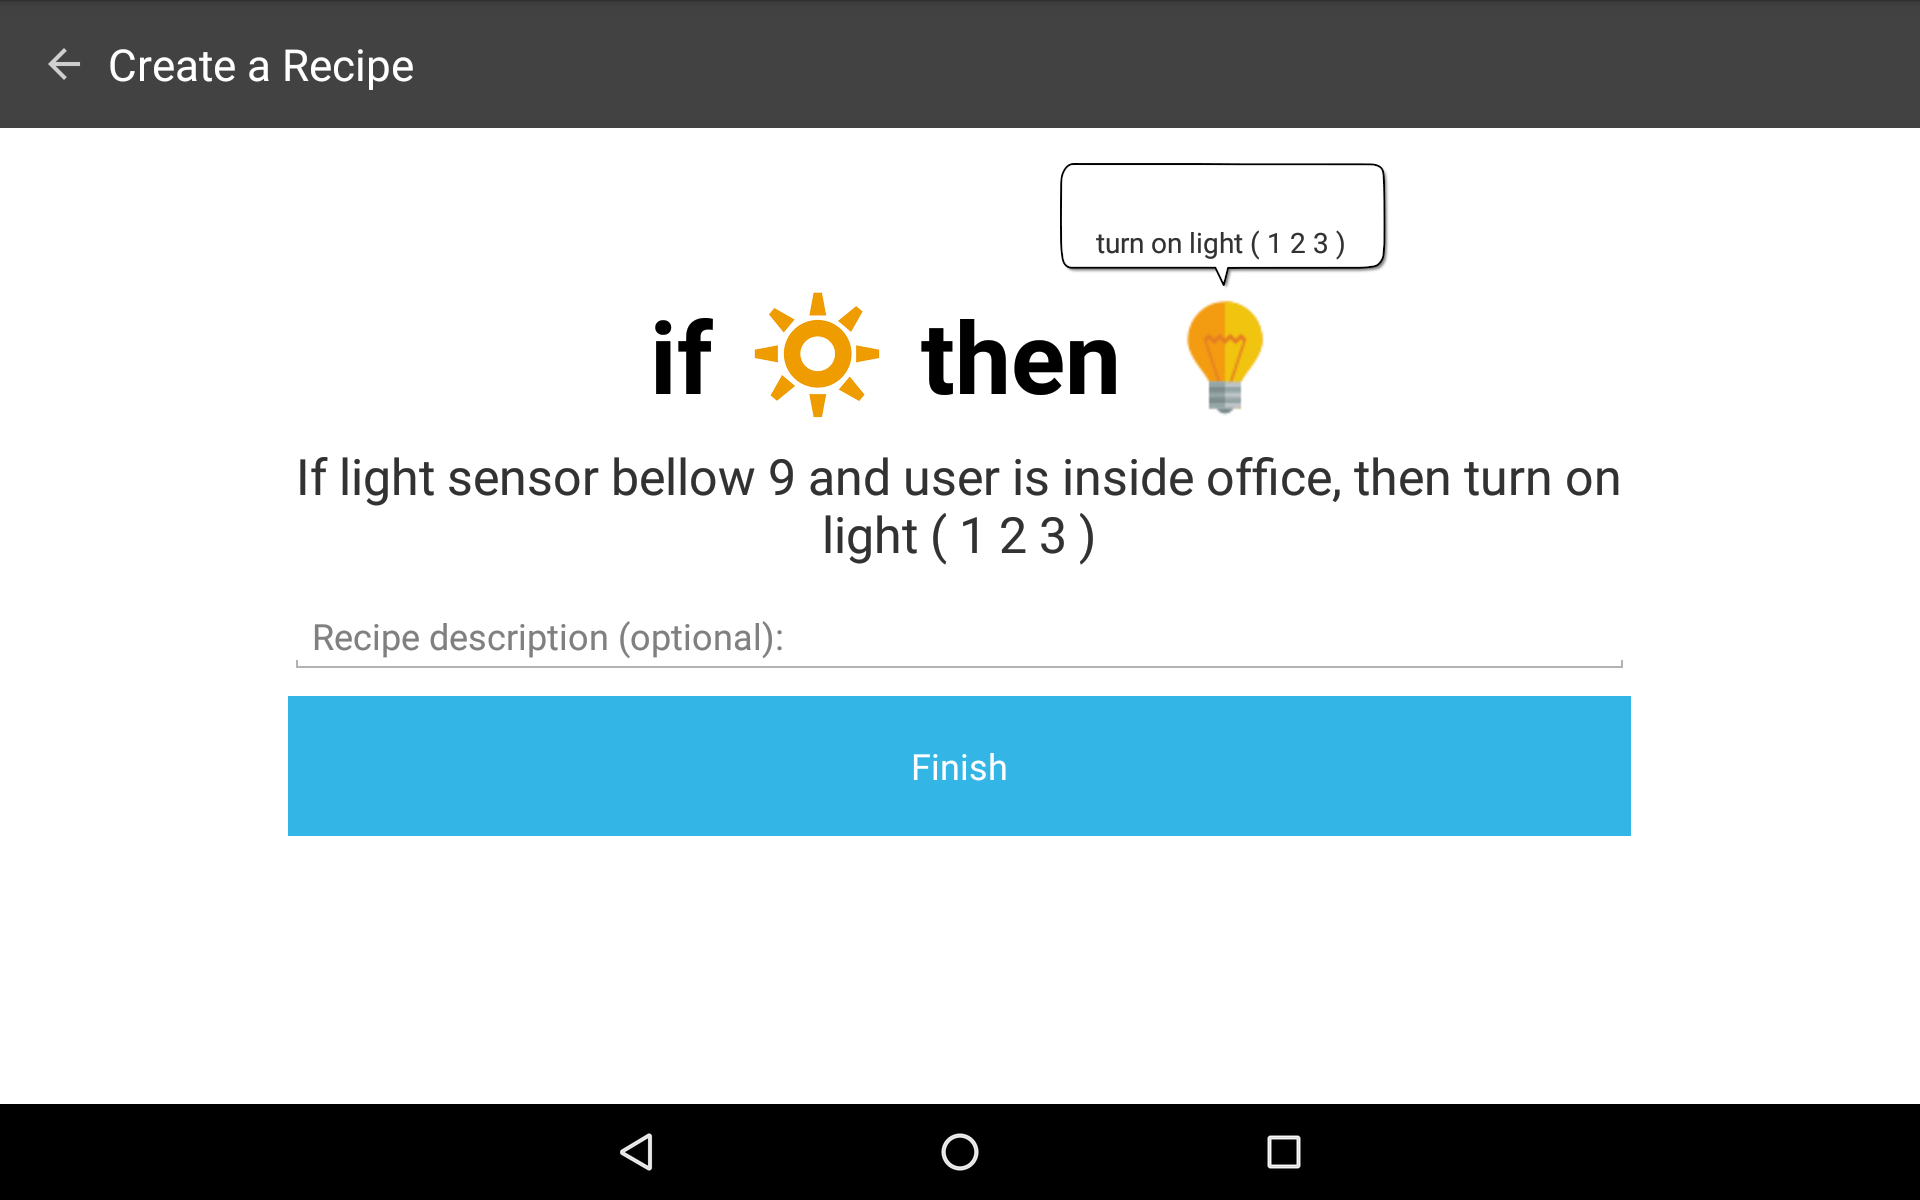
\includegraphics[width=0.6\textwidth]{Figures/screen_completed_recipe}
\caption{Final recipe creation fragment.}
\label{screen_completed_recipe}
\end{figure}



%\begin{figure}[h]
%\centering
%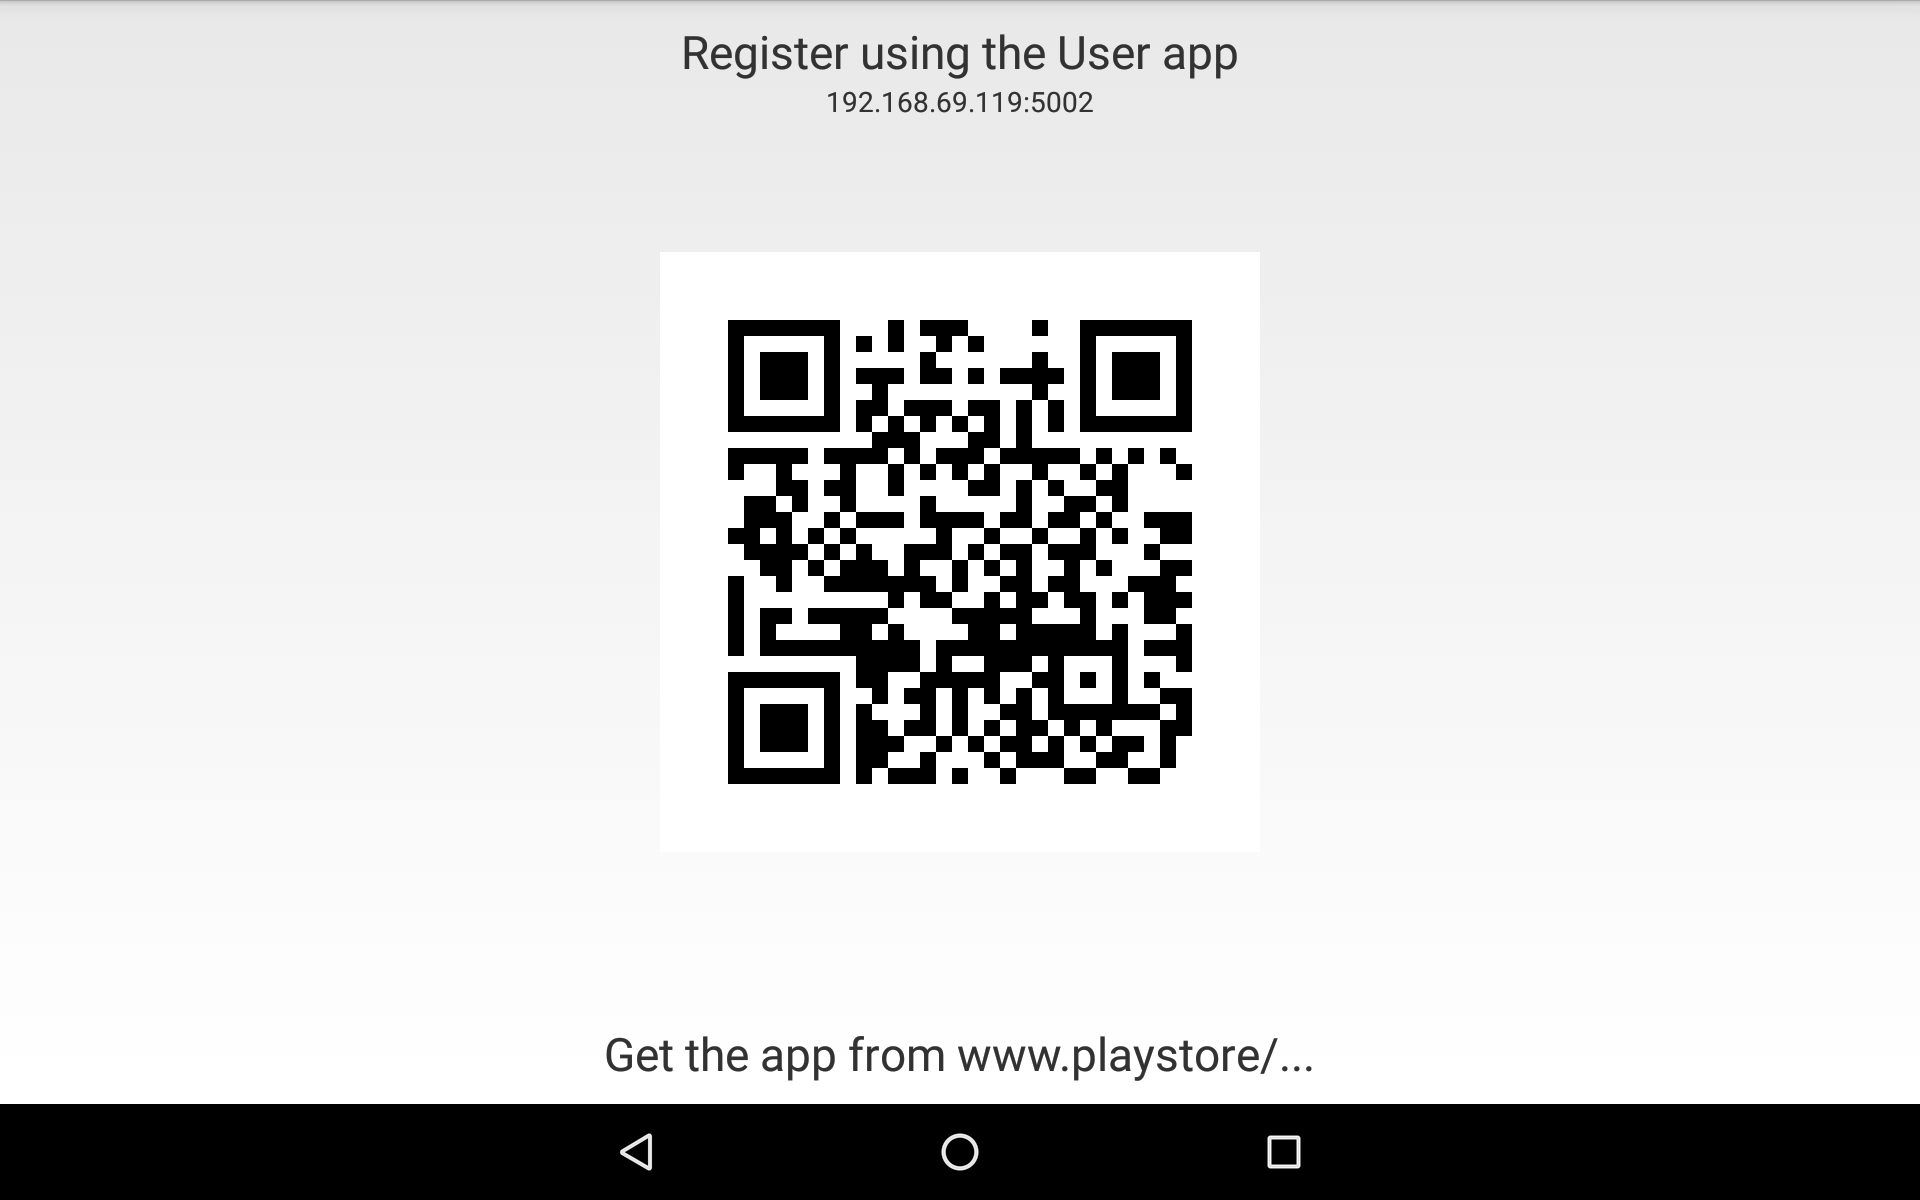
\includegraphics[width=0.7\textwidth]{Figures/screen_qr_code}
%\caption{Registration screen when using USER APP.}
%\label{screen_qr_code}
%\end{figure}


\subsection{User app}


The User app allows user detection, remote control over the office, access to live image preview of the office, notifications when movement is detected, and video history of recorded videos.

The goal of the applications is to add and control Hub devices. This means a user can add multiple Hubs to a user app and manage them. 

To add a device the first to do is create a zone, shown in Figure~\ref{imp_user_app}, a zone is a virtual representation of a building. For example we can create a zone and name it "Home", then add all our Hub tablets within the household. 

After we created a zone we can add a device. To add a device the user presses the "Add device" button, then a screen with a camera and instructions is shown, as described in Figure~\ref{imp_user_add}. The goal is to register the user in the Hub, to to this the user must first open the registration screen in the Hub and then point the camera in the user's phone to the QR-code shown in the Hub registration screen. Afterwords all the user needs to do is press save and the Hub is added and can be controlled.


When a Hub device is added three icons representing three services appear in the zone screen: control lighting, \ac{HVAC} and security systems. This is shown in Figure~\ref{imp_user_app}.

The lighting and \ac{HVAC} screens are straightforward, they allow the user to remotely control a HUB's lighting and \ac{HVAC} systems. The security screen, shown in Figure~\ref{imp_user_camera} enables live camera visualization of the HUB's camera and a list of recorded videos. When motion is detected by the HUB all registered users are notified via Android notification, the purpose of the live camera is to allow the user to check if someone is indeed inside the office. The recorded video history are small 30 second videos captured when movement was detected and no user was inside the room. They allow the user to check in the future if something happened.


The application has two main screens the UserFragment and the HomeFragment. The UserFragment, shown in Figure~\ref{imp_user_app} allows the user to manage the zones and change application settings. The HomeFragment shows the current selected zone and all its devices.

In the settings screen available through the UserFragment, the user can change some parameters such as enable/disable Firebase and location tracking or scan for wireless APs. The screen to scan for wireless APs allows the application to scan and then share via email the list of \ac{MAC address} used for building location.



\begin{figure}
\centering     %%% not \center
\subfigure[Zone creation screen.]{\label{imp_zone_user_app}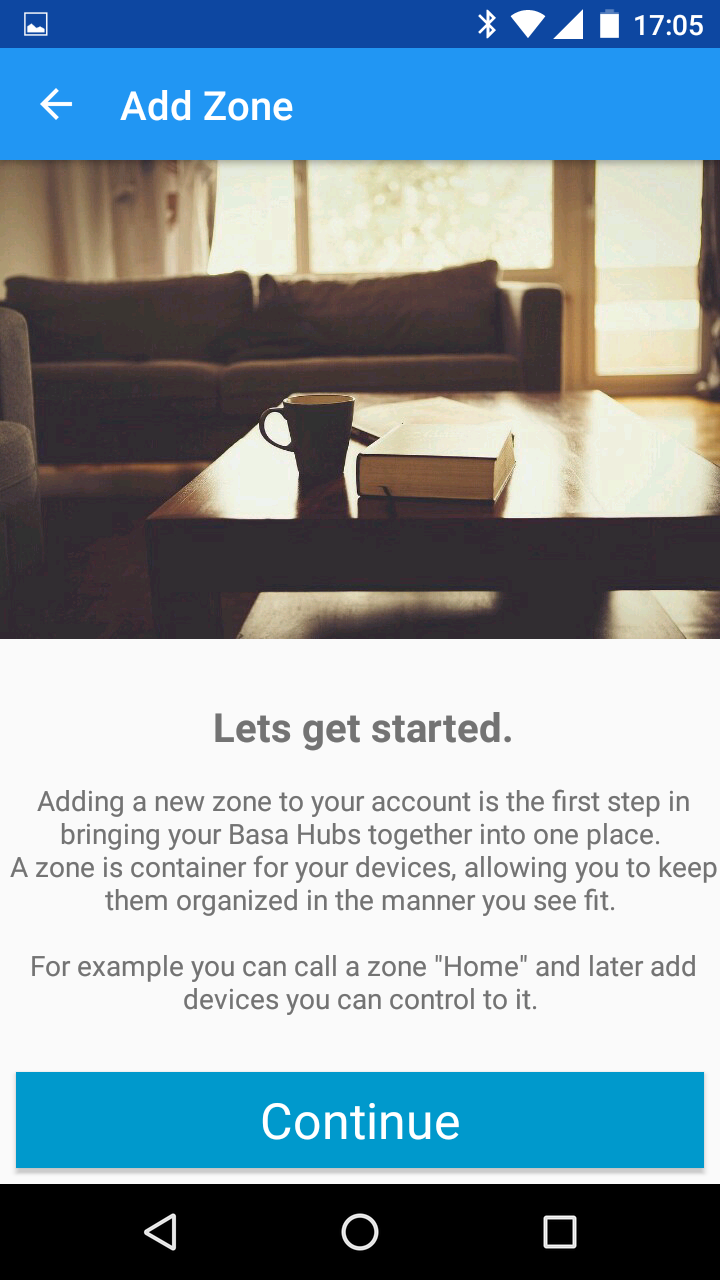
\includegraphics[width=60mm]{Figures/imp_zone_user_app}}
\subfigure[HomeFragment screen with the added Hub.]{\label{imp_home_user_app}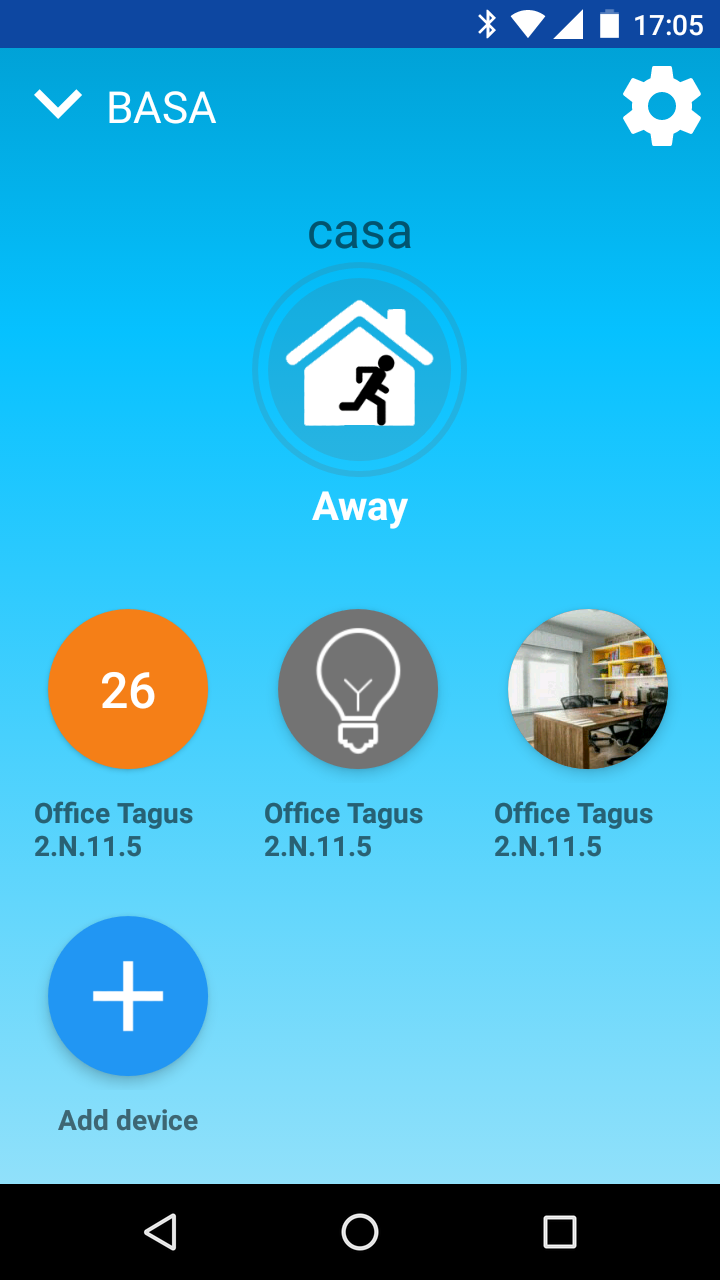
\includegraphics[width=60mm]{Figures/imp_home_user_app}}
\caption{Zone creation and Zone display.}
\label{imp_user_app}
\end{figure}

\begin{figure}
\centering     %%% not \center
\subfigure[Before scan QR-Code of Hub device.]{
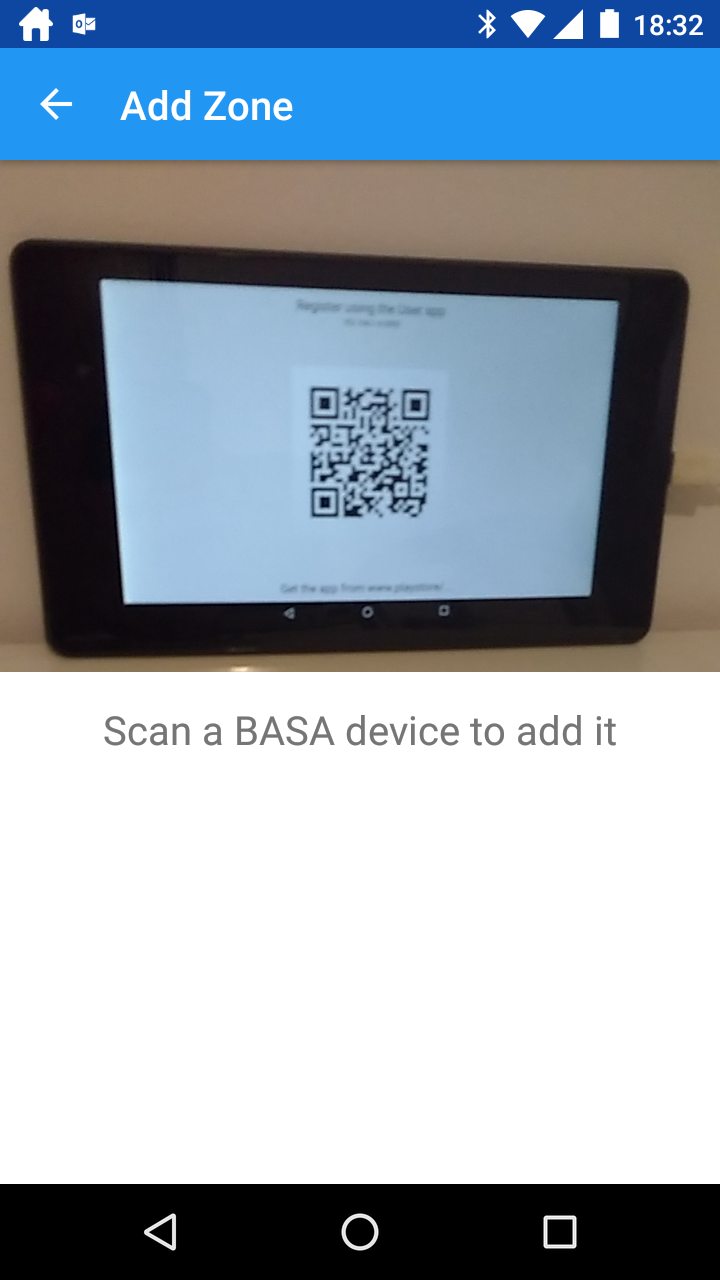
\includegraphics[width=0.35\textwidth]{Figures/imp_user_add_1}}
\subfigure[After scan QR-Code, the device can be added.]{
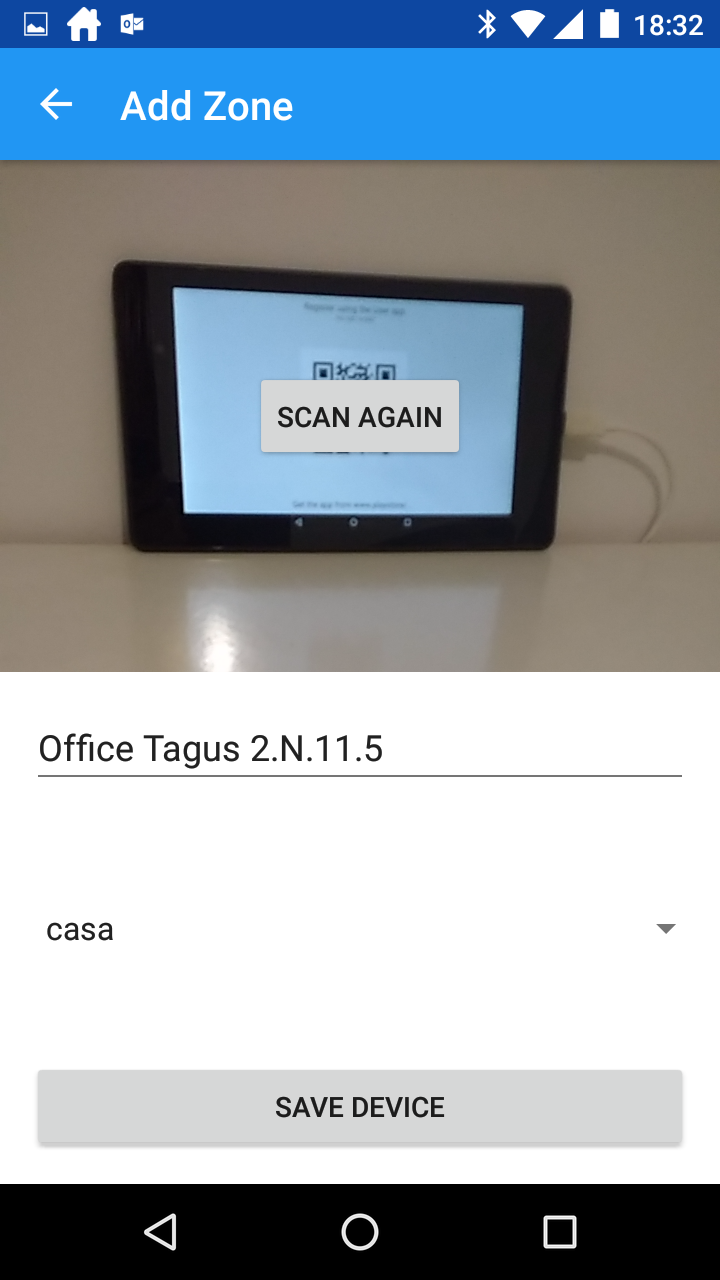
\includegraphics[width=0.35\textwidth]{Figures/imp_user_add_2}}
\caption{Adding a Hub device to the user app.}
\label{imp_user_add}
\end{figure}



\begin{figure}
\centering     %%% not \center
\subfigure[Live camera of the office]{
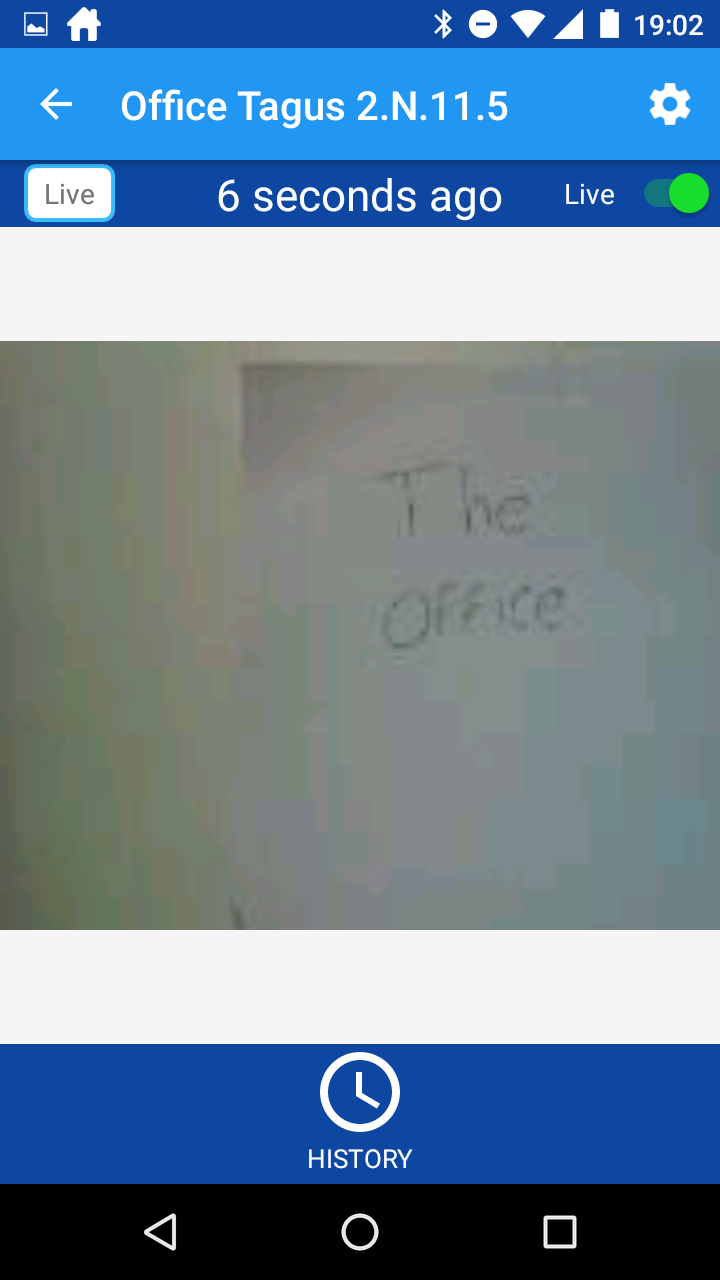
\includegraphics[width=0.35\textwidth]{Figures/imp_user_live}}
\subfigure[Video history, videos when movement was detected]{
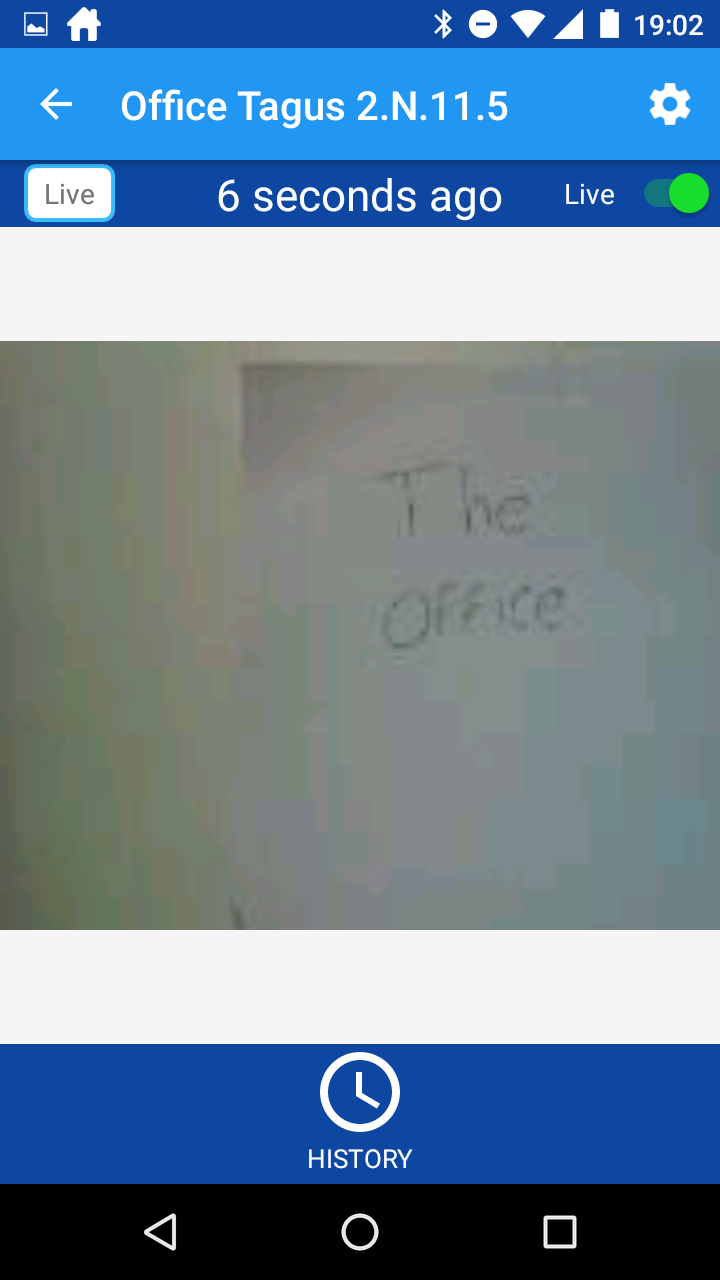
\includegraphics[width=0.35\textwidth]{Figures/imp_user_live}}
\caption{Security - live camera and video history}
\label{imp_user_camera}
\end{figure}




\subsection{Arduino HVAC}


The Arduino we implemented to control the HVAC system was written using C++ programming language. It has four jobs: run a webserver to allow remote control, implement \ac{SSDP} to enable discovery, read temperature/humidity values from a DHT11 sensor and control a four relay module to control de HVAC system.

After the device is first powered up it becomes an \ac{AP}. The user must connect to this new network and use the browser to choose the \ac{WiFi} network he want the Arduino to connect.


The webserver has the following endpoints:


\begin{itemize}
  \item \textbf{GET /:} Shows xml description of the device, used after \ac{SSDP} was performed to list the devices.
  \item \textbf{GET /reset:} Resets the Arduino device, needed if we want to change the WiFi network the Arduino is connected.
  \item \textbf{POST /data} Receives a JSON message to control the HVAC system, for example the message \textit{\{"cha1": 1, "cha2": 0, "cha3": 1, "cha4": 0\}} sends cold air at low speed, more information can be found in Figure~\ref{arduino_post_imp}.
  
  \item \textbf{GET /data} Receives a JSON with the current temperature and humidity.
 
\end{itemize}




